% This must be in the first 5 lines to tell arXiv to use pdfLaTeX, which is strongly recommended.
\pdfoutput=1
% In particular, the hyperref package requires pdfLaTeX in order to break URLs across lines.

\documentclass[11pt]{article}

% Change "review" to "final" to generate the final (sometimes called camera-ready) version.
% Change to "preprint" to generate a non-anonymous version with page numbers.
\usepackage[preprint]{acl}

% Standard package includes
\usepackage{times}
\usepackage{latexsym}

% For proper rendering and hyphenation of words containing Latin characters (including in bib files)
\usepackage[T1]{fontenc}
% For Vietnamese characters
% \usepackage[T5]{fontenc}
% See https://www.latex-project.org/help/documentation/encguide.pdf for other character sets

% This assumes your files are encoded as UTF8
\usepackage[utf8]{inputenc}
\usepackage{tcolorbox}
% This is not strictly necessary, and may be commented out,
% but it will improve the layout of the manuscript,
% and will typically save some space.
\usepackage{microtype}
\usepackage{listings}
\usepackage{amsmath}

\usepackage{xcolor}
\usepackage{listings}

% 定义JSON样式
\lstdefinelanguage{json}{
    basicstyle=\normalfont\ttfamily,
    % numbers=left,
    % numberstyle=\scriptsize,
    % stepnumber=1,
    % numbersep=8pt,
    showstringspaces=false,
    breaklines=true,
    % frame=lines,
    % backgroundcolor=\color{background},
    literate=
        *{0}{{{\color{numb}0}}}{1}
         {1}{{{\color{numb}1}}}{1}
         {2}{{{\color{numb}2}}}{1}
         {3}{{{\color{numb}3}}}{1}
         {4}{{{\color{numb}4}}}{1}
         {5}{{{\color{numb}5}}}{1}
         {6}{{{\color{numb}6}}}{1}
         {7}{{{\color{numb}7}}}{1}
         {8}{{{\color{numb}8}}}{1}
         {9}{{{\color{numb}9}}}{1}
         {:}{{{\color{punct}{:}}}}{1}
         {,}{{{\color{punct}{,}}}}{1}
         {\{}{{{\color{delim}{\{}}}}{1}
         {\}}{{{\color{delim}{\}}}}}{1}
         {[}{{{\color{delim}{[}}}}{1}
         {]}{{{\color{delim}{]}}}}{1},
}


% This is also not strictly necessary, and may be commented out.
% However, it will improve the aesthetics of text in
% the typewriter font.
\usepackage{inconsolata}

%Including images in your LaTeX document requires adding
%additional package(s)
\usepackage{graphicx}
\usepackage{caption}    
\usepackage{subcaption} 
\usepackage{tikz}
\usepackage{pgfplots}
% 添加常用的TikZ库
\usetikzlibrary{
    positioning,         % 用于节点定位
    decorations.markings,% 用于装饰路径的标记
    arrows.meta,         % 更强大的箭头样式
    calc,                % 坐标计算
    patterns,            % 填充图案
    shapes,              % 各种形状
    backgrounds,         % 背景
    fit,                 % 自动调整大小以适应多个节点
    automata,            % 绘制自动机状态图
    petri,               % 绘制 Petri 网
    intersections        % 求交点
}
% \usepackage[active,tightpage]{preview} 
% \PreviewEnvironment{tikzpicture}
% \setlength\PreviewBorder{2mm} % 边距

\newtheorem{corollary}{Corollary}
\newtheorem{prop}{Prop}
% If the title and author information does not fit in the area allocated, uncomment the following
%
%\setlength\titlebox{<dim>}
%
% and set <dim> to something 5cm or larger.

% \title{Verification and Extension of Social Exchange Theory based on LLM Agent

% and of Homans' Social Exchange Theory with LLM based Agents
% }

\title{Investigating and Extending Homans’ Social Exchange Theory \\with Large Language Model based Agents}


% Author information can be set in various styles:
% For several authors from the same institution:
% \author{Author 1 \and ... \and Author n \\
%         Address line \\ ... \\ Address line}
% if the names do not fit well on one line use
%         Author 1 \\ {\bf Author 2} \\ ... \\ {\bf Author n} \\
% For authors from different institutions:
% \author{Author 1 \\ Address line \\  ... \\ Address line
%         \And  ... \And
%         Author n \\ Address line \\ ... \\ Address line}
% To start a separate ``row'' of authors use \AND, as in
% \author{Author 1 \\ Address line \\  ... \\ Address line
%         \AND
%         Author 2 \\ Address line \\ ... \\ Address line \And
%         Author 3 \\ Address line \\ ... \\ Address line}

% \author{First Author \\
%   Affiliation / Address line 1 \\
%   \texttt{email@domain} \\\And
%   Second Author \\
%   Affiliation / Address line 1 \\
%   \texttt{email@domain} \\}

\author{
    \textbf{Lei Wang\textsuperscript{1}},
    \textbf{Zheqing Zhang\textsuperscript{1}},
    \textbf{Xu Chen\textsuperscript{1}\thanks{Corresponding Author}},
\\
\textsuperscript{1}Renmin University of China,
\\
\texttt{\{wanglei154, zhangzheqing, xu.chen\}@ruc.edu.cn}
% \texttt{\{wanglei154, 2020202812, yanqidai, xu.chen, jrwen\}@ruc.edu.cn},\\
% \{jianxun.lian, xingx\}@microsoft.com,\\
% hxli@stu.pku.edu.cn
}

%\author{
%  \textbf{First Author\textsuperscript{1}},
%  \textbf{Second Author\textsuperscript{1,2}},
%  \textbf{Third T. Author\textsuperscript{1}},
%  \textbf{Fourth Author\textsuperscript{1}},
%\\
%  \textbf{Fifth Author\textsuperscript{1,2}},
%  \textbf{Sixth Author\textsuperscript{1}},
%  \textbf{Seventh Author\textsuperscript{1}},
%  \textbf{Eighth Author \textsuperscript{1,2,3,4}},
%\\
%  \textbf{Ninth Author\textsuperscript{1}},
%  \textbf{Tenth Author\textsuperscript{1}},
%  \textbf{Eleventh E. Author\textsuperscript{1,2,3,4,5}},
%  \textbf{Twelfth Author\textsuperscript{1}},
%\\
%  \textbf{Thirteenth Author\textsuperscript{3}},
%  \textbf{Fourteenth F. Author\textsuperscript{2,4}},
%  \textbf{Fifteenth Author\textsuperscript{1}},
%  \textbf{Sixteenth Author\textsuperscript{1}},
%\\
%  \textbf{Seventeenth S. Author\textsuperscript{4,5}},
%  \textbf{Eighteenth Author\textsuperscript{3,4}},
%  \textbf{Nineteenth N. Author\textsuperscript{2,5}},
%  \textbf{Twentieth Author\textsuperscript{1}}
%\\
%\\
%  \textsuperscript{1}Affiliation 1,
%  \textsuperscript{2}Affiliation 2,
%  \textsuperscript{3}Affiliation 3,
%  \textsuperscript{4}Affiliation 4,
%  \textsuperscript{5}Affiliation 5
%\\
%  \small{
%    \textbf{Correspondence:} \href{mailto:email@domain}{email@domain}
%  }
%}

\begin{document}
\maketitle
\begin{abstract}

Homans' Social Exchange Theory (SET) is widely recognized as a basic framework for understanding the formation and emergence of human civilizations and social structures.
In social science, this theory is typically studied based on simple simulation experiments or real-world human studies, both of which either lack realism or are too expensive to control.
In artificial intelligence, recent advances in large language models (LLMs) have shown promising capabilities in simulating human behaviors.
Inspired by these insights, we adopt an interdisciplinary research perspective and propose using LLM-based agents to study Homans' SET.
Specifically, we construct a virtual society composed of three LLM agents and have them engage in a social exchange game to observe their behaviors. Through extensive experiments, we found that Homans' SET is well validated in our agent society, demonstrating the consistency between the agent and human behaviors.
Building on this foundation, we intentionally alter the settings of the agent society to extend the traditional Homans' SET, making it more comprehensive and detailed. To the best of our knowledge, this paper marks the first step in studying Homans' SET with LLM-based agents. More importantly, it introduces a novel and feasible research paradigm that bridges the fields of social science and computer science through LLM-based agents. Code is available at 
%\url{https://anonymous.4open.science/r/SET-1765}.
\url{https://github.com/Paitesanshi/SET}.
\end{abstract}

\section{Introduction}

Exchange behavior has been a fundamental characteristic of human society since ancient times, as people fulfill each other's needs through both material and non-material exchanges. Social Exchange Theory (SET)~\cite{homans1958social}, proposed by George Homans, stands as one of the most fundamental frameworks in social science for understanding human interaction patterns. By conceptualizing social behaviors as exchange processes where individuals seek to maximize their benefits, Homans' SET provides profound insights into the mechanisms underlying human social interactions. Its influence extends far beyond sociology, shaping our understanding of human behavior across multiple disciplines including psychology, organizational behavior, and economics~\cite{blau2017exchange,cropanzano2005social}.


{
In social science, the study of Homans' SET has evolved through two primary methodological approaches. Traditional research relied on real-human studies through empirical observations and laboratory experiments~\cite{cropanzano2017social,orpen1994effects,witt2001interactive}, which have contributed significantly to our understanding but are limited by practical constraints in controlling variables, high resource requirements in both time and cost, and difficulties in replicating exact experimental conditions. To address these limitations, researchers developed simulation-based approaches, particularly Agent-Based Modeling (ABM)~\cite{enayat2022computational}, enabling systematic exploration of exchange dynamics through computational models. However, traditional ABM approaches, constrained by predetermined rules and simple functions, struggle to capture the complexity of human cognitive processes and emotional responses in social exchanges. 
The above limitations naturally raise the question: "Can we develop a new methodology that both captures realistic human behavior and enables flexible experiment control to comprehensively investigate Homans' SET?"
}

\begin{figure*}[t!]
    \centering
    \includegraphics[width=\linewidth]{figs/homans_3.pdf}
    \caption{Illustration and examples of the six propositions in Homans' Social Exchange Theory. }
    \label{fig:main}
\end{figure*}
{
At the same time, in the field of artificial intelligence, researchers have developed numerous cost-effective Large Language Models (LLMs) by training on extensive human-generated corpora. These models have demonstrated remarkable capabilities in natural language understanding and human-like cognitive processing~\cite{kojima2022large,zhao2023survey,achiam2023gpt}.
Inspired by such advantages of LLMs, in this paper, we propose to study Homans' SET with LLM-based agents.
Specifically, We establish an experimental agent society, where different agents can freely exchange resources with each other.
To make each agent behave more like humans, we carefully design an agent framework that can reason and make decisions considering emotional and social factors.
Our agent society is operated in a round-by-round manner, and in each round, there are two phases: \textit{Negotiation}, where the agents discuss exchange arrangements; and \textit{Exchange}, where the agents make individual decisions about resource allocation. 
}

{
Based on above agent society, we first verify Homans' SET by systematically observing and analyzing agent behaviors, where we find that they can well align with the six propositions of Homans' SET, validating the effectiveness of our agents in simulating human behaviors. 
Based on this foundation, we further extend Homans' SET.
Specifically, we investigate how cognitive processing styles and social value orientations influence the interaction dynamics between different humans, and explore the resilience of the social exchange systems. 

In summary, the main contributions of this paper are as follows:
(1) We open the interdisciplinary direction of leveraging LLM-based agents to study Homans' SET.
(2) We design a human-inspired agent framework and a multi-agent society to assist the study of Homans' SET.
(3) We conduct extensive experiments to validate Homans' SET within our agent society, demonstrating that it provides an effective environment for studying this theory.
(4) We extend Homans' SET, and conduct real-world experiments to verify our extensions.





\section{Preliminary}
{To enhance the clarity of our paper, this section provides a brief introduction to Homans' SET.
In general, Homans' SET conceptualizes human social behaviors as exchange processes where individuals assess rewards and costs in social interactions. 
More specifically, there are six core propositions:}

\begin{prop}
[\textbf{Success Proposition}]
This proposition suggests that a rewarded action is more likely to be repeated in the following behaviors. 
\end{prop}
For example, if a person successfully exchanges resources with another, they may be inclined to exchange with the same partner again (Figure~\ref{fig:main}(a)).

\begin{prop}
[\textbf{Stimulus Proposition}] 
This proposition suggests that similar stimuli to those associated with past rewards trigger similar actions. 
\end{prop}
For example, when people need specific resources, they tend to seek out partners who provided them successfully before (Figure~\ref{fig:main}(b)).

\begin{prop}
[\textbf{Value Proposition}]
This proposition suggests that more valuable outcomes increase the likelihood of a human action.
\end{prop}
For example, people tend to seek combinations of different resources that yield greater value, rather than accumulating single resource (Figure~\ref{fig:main}(c)).

\begin{prop}
[\textbf{Deprivation–Satiation Proposition}]
This proposition suggests that the value of a reward diminishes with frequent recent receipt. 
\end{prop}
For example, when a person accumulates an excess of one resource in a short period, they prioritize acquiring the resources they lack (Figure~\ref{fig:main}(d)).

\begin{prop}
[\textbf{Aggression–Approval Proposition}]
This proposition suggests that unexpected punishment leads to anger behavior, while unexpected rewards or avoided punishment elicit approval. 
\end{prop}
For example, people usually express different emotional responses to over-delivery or under-delivery in exchanges (Figure~\ref{fig:main}(e)).

\begin{prop}
[\textbf{Rationality Proposition}]
This proposition suggests that people choose actions with the highest expected value based on past experience and perceived probability of success. 
\end{prop}
For example. people may balance potential profits against transaction reliability when selecting trading partners (Figure~\ref{fig:main}(f)).

The above six propositions form the core of Homans' SET, revealing the fundamental decision-making patterns behind human social behavior. Traditionally, this theory has been widely studied in social science through simple simulation methods or real-human studies, which are either too far from realistic or costly and difficult to control. 
In the following, we leverage LLM-based agents to investigate and extend traditional Homans' SET, offering a more efficient way to study this theory.



\section{The Constructed Agent Society}

\subsection{Single Agent Framework}
{Since Homans' SET building on social exchange emphasizes complex interpersonal dynamics and intrinsic psychological processes, traditional agent frameworks designed for general purposes may not effectively capture these nuanced behaviors.
As a result, we build a tailored agent framework for social exchange, which highlights the following four components:
}

$\bullet$ \textbf{Belief-Desire-Intention (BDI)}. 
To accurately simulate human analytical capabilities, we adopt the BDI framework to model agents' decision-making processes~\cite{georgeff1999belief}, where \textit{Belief} represents the agent’s understanding of its own resources, \textit{Desire} defines the agent’s target objectives, and \textit{Intention} outlines the action plans the agent intends to pursue.

$\bullet$ \textbf{Affinity}.
In real-world social exchange behaviors, psychological factors can significantly influence human decisions~\cite{skinner2019behavior}. To model this phenomenon, we maintain an emotional score for each agent toward others based on their interaction history. These scores evolve dynamically: they increase when exchanges are reciprocal and beneficial, and decrease when agents experience unfair exchanges or breaches of commitment.

$\bullet$ \textbf{Rational-Experiential Inventory (REI)}.
In practice, people may exchange resources with others based on both rational and experiential thinking styles. To flexibly balance these styles, we introduce the REI framework~\cite{keaton2017rational}, where each agent is assigned two scores ranging from 1 to 5: a rational score that quantifies analytical capacity and an experiential score that measures reliance on intuition and past experiences. 

% To create distinct behavioral patterns, we configure rationally-oriented agents with a rational score of 5 and experiential score of 1, while experientially-oriented agents receive the opposite configuration. This design allows us to systematically study how different thinking styles influence exchange behaviors.

% where rational thinking is modeled through BDI and experiential thinking through affinity

% We evaluate various LLMs using the REI-40 questionnaire~\cite{keaton2017rational} to understand their cognitive preferences. Results in Figure~\ref{fig:rei_result} show different models exhibit distinct preferences, indicating the need to explicitly calibrate the rational-experiential balance in our agent architecture.

$\bullet$ \textbf{Social Value Orientation (SVO)}. 
Value orientations fundamentally shape behavioral patterns in social exchanges. To model such factors, we draw on established research~\cite{bogaert2008social} and classify agents into two categories: Proself agents who optimize for individual utility maximization, and Prosocial agents who pursue reciprocal benefits in interactions. These agent types are implemented through pre-defined LLM prompting templates.

% equipped with a profile describes their decision-making style and behavioral preferences.


% Based on the SVO framework~\cite{bogaert2008social}, we classify agents as either Proself who maximize own outcomes or Prosocial who balance self and others' benefits. 


% To understand the inherent social preferences of different LLMs, we evaluate them using the SVO Slider Measure~\cite{murphy2011measuring}, with results shown in Figure~\ref{fig:svo_result}.

In addition to the above components, each agent maintains a memory module that tracks the complete interaction history of negotiations and exchanges with other agents.
% Furthermore, we require the agents to document the reasoning behind each decision, which remains private and inaccessible to other agents, allowing us to analyze their decision-making processes.

\begin{figure*}[t!]
    \centering
    \includegraphics[width=\linewidth]{figs/main_3.pdf}
    \caption{Overview of the agent society: single agent framework and multi-agent exchange pipeline. }
    \label{fig:pipeline}
\end{figure*}


\subsection{Multi-Agent Society}
{
Building upon the above agent framework, we implement a multi-agent society to validate and extend Homans' SET. 
This virtual society involves $M$ agents, who can exchange $N$ distinct types of resources. 
Each agent starts with an equal allocation of initial resources and receives $S$ units of their specialized resource at the beginning of each round. 
To promote social exchange behavior, we design a value system where resource combinations generate higher value.
For example, a single unit of any resource is worth $r_{1}$, combinations of any two resources yield $r_{2}$, and three different types of resources are worth $r_{3}$.
Resources accumulate as time passes, allowing agents to build up their inventory. The goal of the agents is to maximize their total resource value.}


The agent society is executed in a round-by-round manner, and in each round, there are two sequential phases:
(1) In the negotiation phase, agents engage in up to three rounds of discussions, where they can propose exchanges with specified resource types and quantities, respond to existing proposals, or pass their turn. The communication follows a structured format as presented in Figure~\ref{fig:pipeline}. The phase ends when either three rounds are completed or all agents choose to pass.
(2) In the exchange phase, agents independently decide how to allocate their resources. These decisions are made simultaneously, and agents are free to honor or deviate from their commitments made during negotiations. After the exchange is completed, all actions and outcomes are revealed to all agents.

After each round, the agents update their BDI module as well as their affinity scores toward other agents based on both negotiation behavior and exchange outcomes. 
We conduct experiments over 10 rounds, recording all agent actions and resource dynamics for comprehensive analysis. 

% This controlled environment enables systematic investigation of social exchange patterns while maintaining experimental reproducibility.


\begin{figure*}[!t]
\centering
\begin{subfigure}[b]{0.48\textwidth}
\centering
%\includegraphics[width=\textwidth]{figs/volume.pdf}
% This file was created with tikzplotlib v0.10.1.
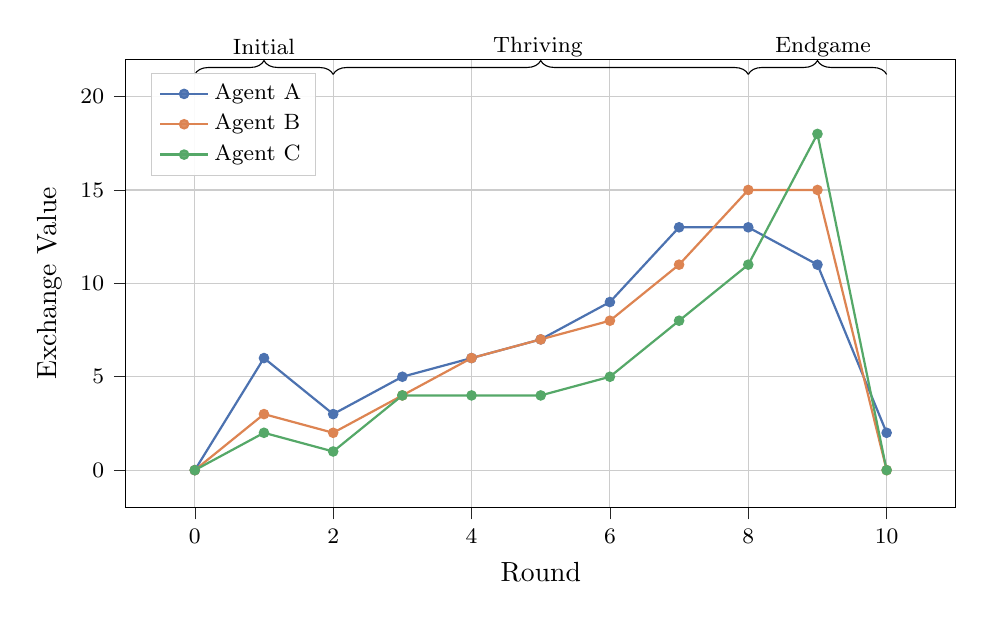
\begin{tikzpicture}

\definecolor{darkorange25512714}{RGB}{221,132,82}
\definecolor{darkslategrey38}{RGB}{38,38,38}
\definecolor{forestgreen4416044}{RGB}{85,168,104}
\definecolor{lightgrey204}{RGB}{204,204,204}
\definecolor{steelblue31119180}{RGB}{76,114,176}


\begin{axis}[
legend cell align={left},
legend style={
  fill opacity=0.8,
  draw opacity=1,
  text opacity=1,
  at={(0.03,0.97)},
  anchor=north west,
  draw=lightgrey204,
  font=\footnotesize
},
width=1.\textwidth,    % 设置宽度
    height=0.6\textwidth,  % 16:9比例
    axis line style={black},
    legend style={fill opacity=0.9, draw opacity=1, text opacity=1, draw=lightgrey204},
    tick align=outside,     % 刻度线向外
    xtick={0,2,4,6,8,10},
    % xticklabels={Initial,Flourishing,Endgame},
     xlabel=Round,
    xlabel style={font=\footnotesize},
    xticklabel style={font=\footnotesize},
    y grid style={lightgrey204},
    ylabel=Exchange Value,
   ylabel style={font=\footnotesize,
            inner sep=0pt,    % 减少标签和轴的距离
            yshift=-12pt       % 微调标签位置
        },
    ymajorgrids,
    ytick={0,5,10,15,20},
    yticklabel style={font=\footnotesize},
    ymin=0, ymax=20,
    xtick style={color=darkslategrey38},
    ytick style={color=darkslategrey38},
    enlarge x limits=0.1,
    enlarge y limits=0.1,
    grid=major,
    grid style={lightgrey204},
    tick style={color=darkslategrey38},
    axis lines=box,        % 保持完整边框
    x axis line style={black},
    y axis line style={black},
    % 控制刻度线的显示
    tick pos=left,         % y轴刻度线只在左侧显示
    xtick pos=bottom,      % x轴刻度线只在底部显示
    clip=false              % 裁剪超出的内容
]
\addplot [thick, steelblue31119180, mark=*, mark size=1.5, mark options={solid}]
table {%
0 0
1 6
2 3
3 5
4 6
5 7
6 9
7 13
8 13
9 11
10 2
};
\addlegendentry{Agent A}
\addplot [thick, darkorange25512714, mark=*, mark size=1.5, mark options={solid}]
table {%
0 0
1 3
2 2
3 4
4 6
5 7
6 8
7 11
8 15
9 15
10 0
};
\addlegendentry{Agent B}
\addplot [thick, forestgreen4416044, mark=*, mark size=1.5, mark options={solid}]
table {%
0 0
1 2
2 1
3 4
4 4
5 4
6 5
7 8
8 11
9 18
10 0
};
\addlegendentry{Agent C}

\draw [decorate, decoration={brace, amplitude=5pt},yshift=8pt] (axis cs:0,20) -- (axis cs:2,20) node [black,midway,yshift=10pt, font=\tiny] {\footnotesize Initial};
\draw [decorate, decoration={brace, amplitude=5pt},yshift=8pt] (axis cs:2,20) -- (axis cs:8,20) node [black,midway,yshift=10pt, font=\tiny,xshift=-1pt] {\footnotesize Thriving};
\draw [decorate, decoration={brace, amplitude=5pt},yshift=8pt] (axis cs:8,20) -- (axis cs:10,20) node [black,midway,yshift=10pt, font=\tiny,xshift=2pt] {\footnotesize Endgame};

\end{axis}

\end{tikzpicture}

\caption{Per-round exchange value of each agent.}
\label{fig:case_value}
\end{subfigure}
\hfill
\begin{subfigure}[b]{0.48\textwidth}
\centering
%\includegraphics[width=\textwidth]{figs/affinity.pdf}
% This file was created with tikzplotlib v0.10.1.
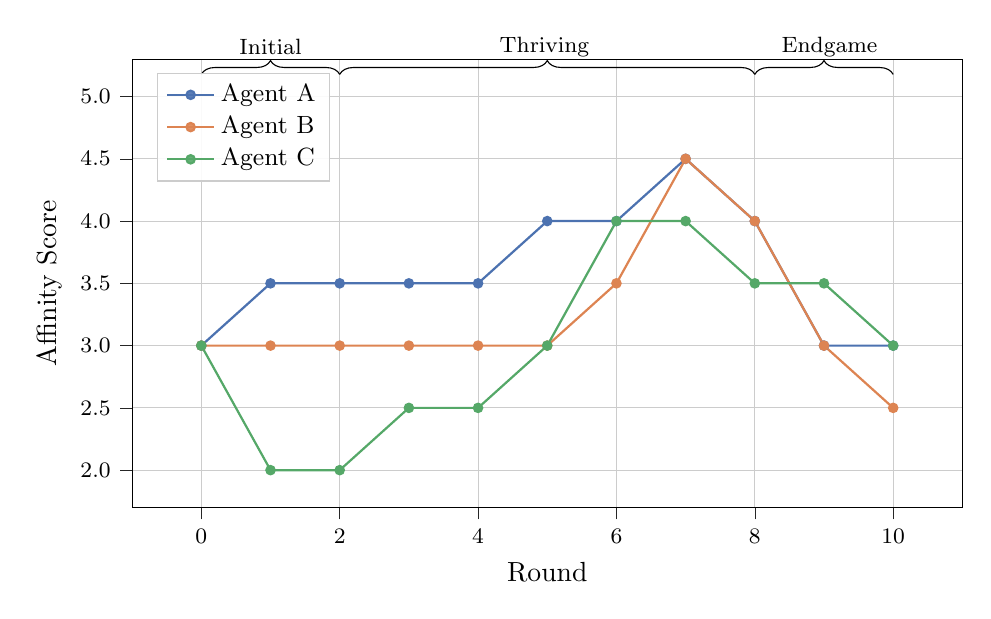
\begin{tikzpicture}

\definecolor{darkslategrey38}{RGB}{38,38,38}
\definecolor{lightgrey204}{RGB}{204,204,204}
\definecolor{mediumseagreen85168104}{RGB}{85,168,104}
\definecolor{peru22113282}{RGB}{221,132,82}
\definecolor{steelblue76114176}{RGB}{76,114,176}

% \begin{axis}[
% axis line style={lightgrey204},
% legend cell align={left},
% legend style={fill opacity=0.8, draw opacity=1, text opacity=1, draw=lightgrey204},
% tick align=outside,
% title={Average Affinity Rating},
% x grid style={lightgrey204},
% xmajorgrids,
% xmajorticks=false,
% xmin=-0.5, xmax=10.5,
% xtick style={color=darkslategrey38},
% y grid style={lightgrey204},
% ylabel=\textcolor{darkslategrey38}{Mean Rating},
% ymajorgrids,
% ymajorticks=false,
% ymin=1.875, ymax=4.625,
% ytick style={color=darkslategrey38}
% ]
\begin{axis}[
legend cell align={left},
legend style={
  fill opacity=0.8,
  draw opacity=1,
  text opacity=1,
  at={(0.03,0.97)},
  anchor=north west,
  draw=lightgrey204,
  font=\small
},
width=1.\textwidth,    % 设置宽度
    height=0.6\textwidth,  % 16:9比例
    axis line style={black},
    legend style={fill opacity=0.9, draw opacity=1, text opacity=1, draw=lightgrey204},
    tick align=outside,     % 刻度线向外
    xtick={0,2,4,6,8,10},
    % xticklabels={Initial,Flourishing,Endgame},
    xticklabel style={font=\footnotesize},
    y grid style={lightgrey204},
    xlabel=Round,
    xlabel style={font=\footnotesize},
    ylabel=Affinity Score,
   ylabel style={font=\footnotesize,
            inner sep=0pt,    % 减少标签和轴的距离
            yshift=-5pt       % 微调标签位置
        },
    ymajorgrids,
    ytick={2.0,2.5,3.0,3.5,4.0,4.5,5.0},
    yticklabel style={font=\footnotesize,
    /pgf/number format/.cd,
    fixed,
    precision=1,
    zerofill},
    ymin=2, ymax=5,
    xtick style={color=darkslategrey38},
    ytick style={color=darkslategrey38},
    enlarge x limits=0.1,
    enlarge y limits=0.1,
    grid=major,
    grid style={lightgrey204},
    tick style={color=darkslategrey38},
    axis lines=box,        % 保持完整边框
    x axis line style={black},
    y axis line style={black},
    % 控制刻度线的显示
    tick pos=left,         % y轴刻度线只在左侧显示
    xtick pos=bottom,      % x轴刻度线只在底部显示
    clip=false              % 裁剪超出的内容
]
\addplot [thick, steelblue76114176, mark=*, mark size=1.5, mark options={solid}]
table {%
0 3
1 3.5
2 3.5
3 3.5
4 3.5
5 4
6 4
7 4.5
8 4
9 3
10 3
};
\addlegendentry{Agent A}
\addplot [thick, peru22113282, mark=*, mark size=1.5, mark options={solid}]
table {%
0 3
1 3
2 3
3 3
4 3
5 3
6 3.5
7 4.5
8 4
9 3
10 2.5
};
\addlegendentry{Agent B}
\addplot [thick, mediumseagreen85168104, mark=*, mark size=1.5, mark options={solid}]
table {%
0 3
1 2
2 2
3 2.5
4 2.5
5 3
6 4
7 4
8 3.5
9 3.5
10 3
};
\addlegendentry{Agent C}

\draw [decorate, decoration={brace, amplitude=5pt},yshift=8pt] (axis cs:0,5) -- (axis cs:2,5) node [black,midway,yshift=10pt, font=\tiny] {\footnotesize Initial};
\draw [decorate, decoration={brace, amplitude=5pt},yshift=8pt] (axis cs:2,5) -- (axis cs:8,5) node [black,midway,yshift=10pt, font=\tiny,xshift=-1pt] {\footnotesize Thriving};
\draw [decorate, decoration={brace, amplitude=5pt},yshift=8pt] (axis cs:8,5) -- (axis cs:10,5) node [black,midway,yshift=10pt, font=\tiny,xshift=2pt] {\footnotesize Endgame};

\end{axis}

\end{tikzpicture}

\caption{Average affinity scores of agents.}
\label{fig:case_affinity}
\end{subfigure}
\caption{Key metrics of agent behavior over 10 rounds.}
\label{fig:case}
\end{figure*}

\section{Validation of Homans' SET}\label{sec:validation}
In this section, we evaluate whether the six propositions of Homans' SET, which have been widely validated in real-human societies~\cite{cook1987social,mighfar2015social}, also hold in our agent society.
In our experiments, the number of resources and agents are both set as 3, that is, $M=N=3$. The value coefficients $r_{1}$, $r_{2}$ and $r_{3}$ are set as 1, 4 and 9, respectively. Initially, each agent has 5 units of each resource type. At the beginning of each round, agents receive 15 units ($S=15$) of their specialized resource.
We use Claude-3.5-sonnet as the base LLM for all agents due to its superior instruction-following capability. 
To remove the randomness, each experiment is repeated for five times, and we report the average results and their standard errors. 
For more experiment settings, we refer the readers to Appendix~\ref{sec:details} for more details.
% For more detailed settings, we refer the readers to our project, which has been released at {xxx}

% To demonstrate the emergent behavioral patterns in our framework, we present a detailed case study that exemplifies the key characteristics observed across experiments. 
% Figure~\ref{fig:case} reveals three distinct phases in the exchange process: initial exploration, relationship building, and strategic adaptation. Each phase demonstrates unique behavioral patterns that reflect the agents' evolving decision-making strategies.

Before introducing the results of validating Homans' SET, we first present a general analysis of the simulation process of our agent society. While the following observations are drawn from comprehensive experimental data, we illustrate the key patterns through a representative case study for better interpretation.
In general, there are three distinct phases (see Figure~\ref{fig:case}).
In the \textbf{initial exploration phase}, the agents exhibited cautious behavior due to the lack of interaction history, engaging in small-scale exchanges to probe counterparts' reliability and preferences. 
In the \textbf{thriving cooperation phase}, agents developed sophisticated exchange strategies based on learned preferences and trust levels. Figure~\ref{fig:case_value} shows a clear positive feedback loop: higher affinity scores enabled larger exchanges, while successful transactions strengthened inter-agent trust.
In the \textbf{strategic endgame phase}, the agents demonstrated sophisticated strategic adaptation. Consistent with the Endgame effect~\cite{adorno1982trying}, agents shifted strategies in final rounds, prioritizing individual utility over relationship maintenance, which is evidenced by decreased exchange values and increased commitment breaches. Figure~\ref{fig:case_affinity} shows the average affinity score each agent received from others. The declining affinity scores reflect this strategic shift from cooperation to self-interest, demonstrating how LLM agents can emulate human-like decision-making in dynamically balancing between collaborative and individualistic behaviors.

With the above intuitive understandings of our agent society, we now systematically validate the Homans' SET propositions as follows:

\textbf{Validation on the Success and Value Propositions}.
% The evolution of exchange value across different phases, as shown in Figure~\ref{fig:volume_distribution}, provides strong evidence for both the Success Proposition and Value Proposition. Initially, agents demonstrate cautious behavior with relatively small exchange value, reflecting their initial risk assessment strategy. As positive exchange experiences accumulate, we observe a significant increase in exchange value during the thriving phase. The violin plot reveals a gradual shift from a concentrated distribution around lower value to a right-skewed distribution, indicating how successful exchanges reinforce exchange strategies and encourage more effective exchanges.
The evidence for these propositions is shown in the evolution of exchange value across different phases (see Figure~\ref{fig:volume_distribution}).
% The evolution of exchange value across different phases, as shown in Figure~\ref{fig:volume_distribution}, provides strong evidence for both propositions. 
Initially, agents demonstrate cautious behavior with small exchange values (median = 3.83). The substantial increase during the thriving phase (median = 6.00, 56.5\% increase) validate the Success Proposition by showing how positive experiences lead to more effective exchanges. The endgame phase maintains a high median value (6.50), validating the Value Proposition based on the fact that trustworthy agents sustain high-value exchanges.
% , while defectors' attempts to exploit these exchanges further demonstrate their pursuit of high-value gains.


\textbf{Validation on the Deprivation-Satiation Proposition}.
Figure~\ref{fig:acceptance_rate} demonstrates a clear inverse relationship between resource abundance and proposal acceptance rates, validating the Deprivation-Satiation Proposition. We measure resource abundance as the ratio of a resource's quantity to the average quantity of all resources an agent possesses in each round, categorizing these ratios into quartiles from Scarce to Abundant. The results show acceptance rates of 70\% under resource scarcity, steadily declining to 23\% as resources become abundant. This diminishing willingness to accept additional resources mirrors the law of diminishing marginal utility in human economic behavior, where the perceived value of each additional unit decreases with increasing abundance.

\begin{figure*}[t!]
    \centering
    \begin{subfigure}[t]{0.32\textwidth}
        \centering
        \begin{figure}
    \centering
    \includegraphics[width=\linewidth]{figures/success_dist.pdf}
    \caption{Distribution of properties of good rewrites.}
    \label{fig:success}
\end{figure}
        \caption{Exchange patterns.}
        \label{fig:volume_distribution}
    \end{subfigure}
    \hfill
    \begin{subfigure}[t]{0.32\textwidth}
        \centering
        

% This file was created with tikzplotlib v0.10.1.
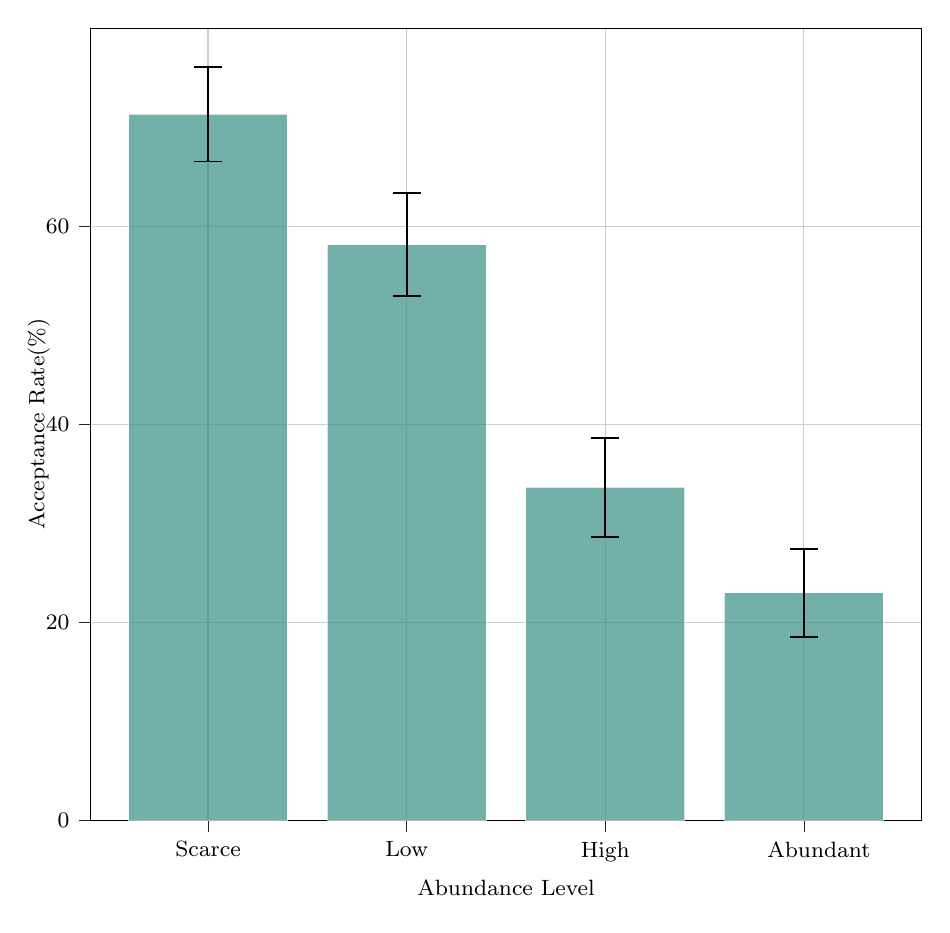
\begin{tikzpicture}

    \definecolor{darkslategrey38}{RGB}{38,38,38}
    \definecolor{darkslategrey66}{RGB}{66,66,66}
    \definecolor{lightgrey204}{RGB}{204,204,204}
    \definecolor{mediumseagreen56142132}{RGB}{56,142,132}
    
    \begin{axis}[
        width=1\textwidth,    % 设置宽度
        height=0.96\textwidth,  % 16:9比例
        axis line style={black},
        tick align=outside,     % 刻度线向外
        axis lines=box,         % 显示完整边框
        tick pos=left,          % y轴刻度线只在左侧
        xtick pos=bottom,       % x轴刻度线只在底部
        clip=true,              % 裁剪超出内容
        unbounded coords=jump,
        x grid style={lightgrey204},
        xlabel=Abundance Level,
        xlabel style={font=\footnotesize},
        xmajorticks=true,
        xmin=-0.59, xmax=3.59,
        xtick style={color=darkslategrey38},
        xtick={0,1,2,3},
        xticklabels={Scarce,Low,High,\hspace{8pt} Abundant},
        xticklabel style={font=\footnotesize,rotate=0},
       % xticklabel 4/.style={xshift=20pt, font=\scriptsize},
        y grid style={lightgrey204},
        ylabel=Acceptance Rate(\%),
        ylabel style={font=\footnotesize ,
            inner sep=0pt,    % 减少标签和轴的距离
            yshift=-5pt       % 微调标签位置
        },
        ymajorgrids,
        ytick={0,20,40,60},  % 添加y轴刻度
        yticklabel style={font=\footnotesize},
        ymin=0, ymax=80,
        ytick style={color=darkslategrey38},
        grid=major,
        grid style={lightgrey204},
        % yticklabel format={\pgfmathprintnumber{#1}},  % 格式化y轴标签
        every outer x axis line/.append style={black},
        every outer y axis line/.append style={black}
    ]
    
  \draw[draw=white,fill=mediumseagreen56142132,opacity=0.7] (axis cs:-0.4,0) rectangle (axis cs:0.4,71.304347826087);
\draw[draw=white,fill=mediumseagreen56142132,opacity=0.7] (axis cs:0.6,0) rectangle (axis cs:1.4,58.1395348837209);
\draw[draw=white,fill=mediumseagreen56142132,opacity=0.7] (axis cs:1.6,0) rectangle (axis cs:2.4,33.6231884057971);
\draw[draw=white,fill=mediumseagreen56142132,opacity=0.7] (axis cs:2.6,0) rectangle (axis cs:3.4,22.9651162790698);
\addplot [line width=0.9pt, darkslategrey66]
table {%
0 nan
0 nan
};
\addplot [line width=0.9pt, darkslategrey66]
table {%
1 nan
1 nan
};
\addplot [line width=0.9pt, darkslategrey66]
table {%
2 nan
2 nan
};
\addplot [line width=0.9pt, darkslategrey66]
table {%
3 nan
3 nan
};
\path [draw=black, semithick]
(axis cs:0,66.5311154292968)
--(axis cs:0,76.0775802228771);

\path [draw=black, semithick]
(axis cs:1,52.9262116653737)
--(axis cs:1,63.3528581020681);

\path [draw=black, semithick]
(axis cs:2,28.6380850776403)
--(axis cs:2,38.6082917339539);

\path [draw=black, semithick]
(axis cs:3,18.5202889931626)
--(axis cs:3,27.4099435649769);

\addplot [semithick, black, mark=-, mark size=5, mark options={solid}, only marks]
table {%
0 66.5311154292968
1 52.9262116653737
2 28.6380850776403
3 18.5202889931626
};
\addplot [semithick, black, mark=-, mark size=5, mark options={solid}, only marks]
table {%
0 76.0775802228771
1 63.3528581020681
2 38.6082917339539
3 27.4099435649769
};
    \end{axis}
    
\end{tikzpicture}
    
        \caption{Resource abundance effect.}
        \label{fig:acceptance_rate}
    \end{subfigure}
    \hfill
    \begin{subfigure}[t]{0.32\textwidth}
        \centering
        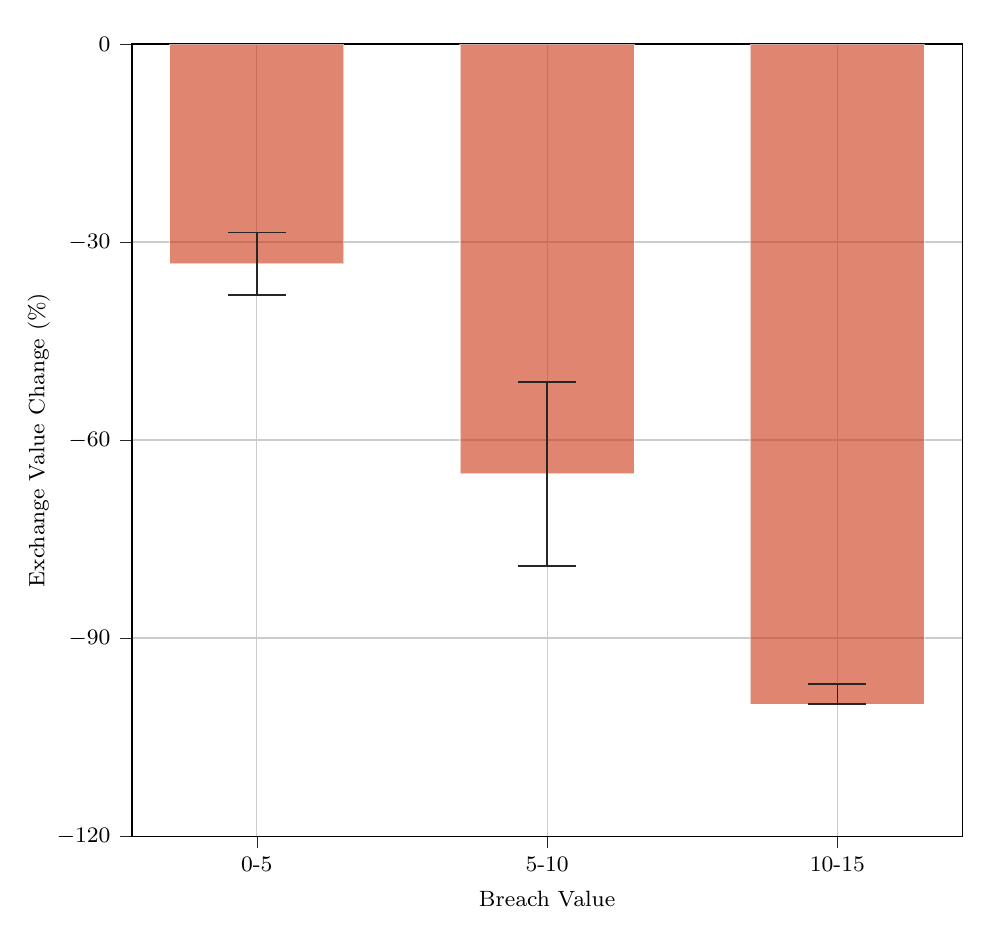
\begin{tikzpicture}
    \definecolor{darkslategrey38}{RGB}{38,38,38}
    \definecolor{darkslategrey66}{RGB}{66,66,66}
    \definecolor{lightgrey204}{RGB}{204,204,204}
    \definecolor{firebrick2045117}{RGB}{204,51,17}
    
    \begin{axis}[
        width=1\textwidth,    % 设置宽度
        height=0.96\textwidth,    % 16:9比例
        axis line style={black},
        tick align=outside,      % 刻度线向外
        anchor=north,
        at={(0,1)}, 
        axis lines=box,          % 显示完整边框
        tick pos=left,           % y轴刻度线只在左侧
        xtick pos=bottom,        % x轴刻度线只在底部
        clip=true,               % 裁剪超出内容
        unbounded coords=jump,
        x grid style={lightgrey204},
        xlabel=Breach Value,
        xlabel style={font=\footnotesize},
        xmajorticks=true,
        xmin=-0.43, xmax=2.43,
        xtick style={color=darkslategrey38},
        xtick={0,1,2},
        xticklabels={0-5,5-10,10-15},
        xticklabel style={font=\footnotesize,rotate=0},
        y grid style={lightgrey204},
        ylabel=Exchange Value Change (\%),
        ylabel style={font=\footnotesize,
            inner sep=0pt,    % 减少标签和轴的距离
            yshift=-1pt       % 微调标签位置
        },
        ymajorgrids,
        ymin=-120, ymax=0,
        ytick={-120,-90,-60,-30,0},
        yticklabel style={font=\footnotesize},
        ytick style={color=darkslategrey38},
        grid=major,
        grid style={lightgrey204},
        every outer x axis line/.append style={black},
        every outer y axis line/.append style={black}
    ]
    
    % 绘制柱状图
    \draw[draw=white,fill=firebrick2045117,opacity=0.6] 
        (axis cs:-0.3,0) rectangle (axis cs:0.3,-33.3017084294457);
    \draw[draw=white,fill=firebrick2045117,opacity=0.6] 
        (axis cs:0.7,0) rectangle (axis cs:1.3,-65.1388888888889);
    \draw[draw=white,fill=firebrick2045117,opacity=0.6] 
        (axis cs:1.7,0) rectangle (axis cs:2.3,-100);
    
    % 误差线
    % \path [draw=darkslategrey38, semithick]
    %     (axis cs:0,-38.0549349367552) -- (axis cs:0,-28.5484819221361);
    % \path [draw=darkslategrey38, semithick]
    %     (axis cs:1,-79.1065317716095) -- (axis cs:1,-51.1712460061683);
    % \path [draw=darkslategrey38, semithick]
    %     (axis cs:2,-97) -- (axis cs:2,-100);
    \draw[darkslategrey38, semithick] (axis cs:-0.1,-38.0549349367552) -- (axis cs:0.1,-38.0549349367552);
    \draw[darkslategrey38, semithick] (axis cs:0,-38.0549349367552) -- (axis cs:0,-28.5484819221361);
    \draw[darkslategrey38, semithick] (axis cs:-0.1,-28.5484819221361) -- (axis cs:0.1,-28.5484819221361);
    
    \draw[darkslategrey38, semithick] (axis cs:0.9,-79.1065317716095) -- (axis cs:1.1,-79.1065317716095);
    \draw[darkslategrey38, semithick] (axis cs:1,-79.1065317716095) -- (axis cs:1,-51.1712460061683);
    \draw[darkslategrey38, semithick] (axis cs:0.9,-51.1712460061683) -- (axis cs:1.1,-51.1712460061683);
    
    \draw[darkslategrey38, semithick] (axis cs:1.9,-97) -- (axis cs:2.1,-97);
    \draw[darkslategrey38, semithick] (axis cs:2,-97) -- (axis cs:2,-100);
    \draw[darkslategrey38, semithick] (axis cs:1.9,-100) -- (axis cs:2.1,-100);
    
    % 百分比标签
    % \node[above,font=\footnotesize\bfseries,text=firebrick2045117] 
    %     at (axis cs:0,-50.3017084294457) {-33.3\%};
    % \node[above,font=\footnotesize\bfseries,text=firebrick2045117] 
    %     at (axis cs:1,-90.1388888888889) {-65.1\%};
    % \node[above,font=\footnotesize\bfseries,text=firebrick2045117] 
    %     at (axis cs:2,-115) {-100.0\%};
        
\end{axis}
\end{tikzpicture}
        \caption{Impact of trust violations.}
        \label{fig:future_proposals}
    \end{subfigure}
        \caption{Experimental validation of key propositions in Social Exchange Theory.}
    \label{fig:set_validation}
\end{figure*}
\textbf{Validation on the Aggression-Approval Proposition}.
The agents' responses to trust violations, depicted in Figure~\ref{fig:future_proposals}, strongly support the Aggression-Approval Proposition. The data reveals a graduated response pattern: minor violations (0-5 breach value) trigger a 33.3\% reduction in future exchanges, moderate breaches (5-10) lead to a 65.1\% decrease, while severe violations (10-15) result in an almost complete cessation of trading relationships (97\% reduction). This proportional punishment mechanism demonstrates how agents develop sophisticated trust management strategies, responding to trust violations with increasing severity as the magnitude of the breach increases.

\textbf{Validation on the Rationality and Stimulus Propositions}.
In general, the agents make decisions by optimizing their values based on accumulated experience and current circumstances, which is consistent with the Rationality Proposition.
For example, in the transition between exchange phases, agents adjust their strategies based on established trust levels and resource requirements. 
In addition, the Stimulus Proposition can be validated through the consistent response patterns observed across similar exchange scenarios, especially during the thriving phase where agents develop stable exchange behaviors under familiar circumstances.

The above experiments collectively demonstrate that all six propositions of Homans' SET can be effectively validated in our agent society, providing a promising foundation for investigating previously unexplored aspects of social exchange theory in human society through LLM-based agents.

\section{Extensions of Homans' SET}
{
A significant advantage of our agent society lies in its flexibility in adjusting agent settings, enabling us to explore Homans' SET under various conditions, which would be prohibitively expensive or even infeasible using traditional real human-based methods.
Leveraging this advantage, we extend traditional Homans' SET by conducting a systematic investigation into how cognitive styles and social value orientations influence exchange behaviors, while also examining the resilience of the social system.
The experiments in this section are conducted based on similar settings to the above section's, and the results are detailed below.
}


\subsection{Cognitive Style}
In this section, we explore how different cognitive styles influence social exchange behaviors. To answer this question, we first set the agents to operate in either a completely rational or a completely experiential manner and then systematically compare their behaviors.
In Figure~\ref{fig:rei_analysis}, we present the average exchange values and affinity scores of the agents in each round.
In general, the results reveal distinct behavioral patterns: rational agents exhibit greater fluctuations in both exchange values and affinity scores, whereas experiential agents demonstrate more stability in these metrics over time.

Actually, these observations are fairly intuitive.
% If the agents are completely experiential, their past behaviors have a strong impact on subsequent decisions. This leads to a high correlation between metrics across successive rounds, resulting in smoother metric curves.
When agents are purely experiential, their past behaviors significantly influence their subsequent decisions, creating strong temporal correlations in their metrics across consecutive rounds. This dependency on historical experiences naturally leads to smoother trajectories in the observed metrics.
On the other hand, if the agents are completely rational, the influence of past behaviors is minimal, causing the metric curves to fluctuate more.
From a broader perspective, this experiment suggests that if a human relies solely on experience to make decisions, their gains will remain stable but are unlikely to reach very high levels.
However, if a human is entirely rational, while they may occasionally achieve very high benefits, they also face the risk of significant losses.

Based on above experimental evidence and analyses, we derive the following corollary further extending Homans' SET:
\begin{corollary}[The Stability Corollary]
In the real world, rational individuals are more likely to achieve higher benefits, but they also face the risk of greater losses. In contrast, individuals with an experiential thinking style tend to achieve more stable but moderate benefits over time.
\end{corollary}









\begin{figure}[t!]
    \centering
    \includegraphics[width=\linewidth]{figs/rei_analysis.pdf}
    %% This file was created with tikzplotlib v0.10.1.
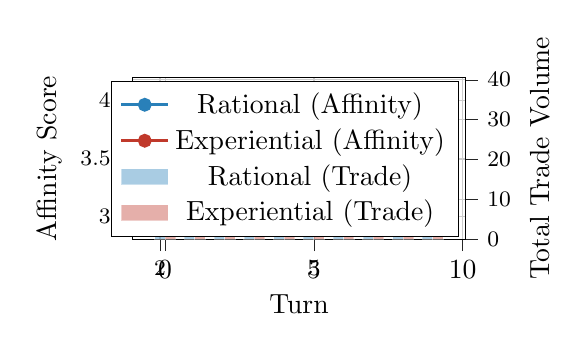
\begin{tikzpicture}

\definecolor{darkslategrey38}{RGB}{38,38,38}
\definecolor{firebrick1925743}{RGB}{192,57,43}
\definecolor{lightgrey204}{RGB}{204,204,204}
\definecolor{steelblue41128185}{RGB}{41,128,185}

\begin{axis}[
   width=0.48\textwidth,
   height=0.3\textwidth,
   axis line style={black},
   tick align=outside,
   x grid style={lightgrey204},
   xlabel=Turn,
   xlabel style={font=\footnotesize, yshift=5pt},
   %xtick={0,1,2,3,4,5,6,7,8,9},
   xticklabels={1,2,3,4,5,6,7,8,9,10},
   xticklabel style={font=\footnotesize},
   ylabel=Affinity Score,
   ylabel style={font=\footnotesize, inner sep=0pt, yshift=-5pt},
   ymajorgrids,
   ymin=2.8, ymax=4.2,
   yticklabel style={font=\footnotesize},
   grid=major,
   grid style={lightgrey204},
   tick style={color=darkslategrey38},
   axis lines=box,
   x axis line style={black},
   y axis line style={black},
   tick pos=left,
   xtick pos=bottom,
   clip=true
]
\path [draw=steelblue41128185, fill=steelblue41128185, opacity=0.2]
(axis cs:0,3.6)
--(axis cs:0,3.25)
--(axis cs:1,3.4)
--(axis cs:2,3.48333333333333)
--(axis cs:3,3.66666666666667)
--(axis cs:4,3.56666666666667)
--(axis cs:5,3.4)
--(axis cs:6,3.36625)
--(axis cs:7,3.21666666666667)
--(axis cs:8,3.16666666666667)
--(axis cs:9,3.08333333333333)
--(axis cs:9,3.68333333333333)
--(axis cs:9,3.68333333333333)
--(axis cs:8,3.78333333333333)
--(axis cs:7,3.81666666666667)
--(axis cs:6,3.9)
--(axis cs:5,3.90041666666667)
--(axis cs:4,4.03333333333333)
--(axis cs:3,4.08333333333333)
--(axis cs:2,3.85)
--(axis cs:1,3.78333333333333)
--(axis cs:0,3.6)
--cycle;

\path [draw=firebrick1925743, fill=firebrick1925743, opacity=0.2]
(axis cs:0,3.56666666666667)
--(axis cs:0,3.19958333333333)
--(axis cs:1,3.11666666666667)
--(axis cs:2,3.05)
--(axis cs:3,3.1)
--(axis cs:4,3.2)
--(axis cs:5,3.33333333333333)
--(axis cs:6,3.3)
--(axis cs:7,3.29958333333333)
--(axis cs:8,3.15)
--(axis cs:9,3.15)
--(axis cs:9,3.75)
--(axis cs:9,3.75)
--(axis cs:8,3.68333333333333)
--(axis cs:7,3.88333333333333)
--(axis cs:6,3.91666666666667)
--(axis cs:5,3.86666666666667)
--(axis cs:4,3.75)
--(axis cs:3,3.58333333333333)
--(axis cs:2,3.5)
--(axis cs:1,3.53333333333333)
--(axis cs:0,3.56666666666667)
--cycle;

\addplot [line width=1pt, steelblue41128185, mark=*, mark size=3, mark options={solid,draw=white}]
table {%
0 3.43333333333333
1 3.6
2 3.66666666666667
3 3.88333333333333
4 3.8
5 3.66666666666667
6 3.63333333333333
7 3.5
8 3.46666666666667
9 3.38333333333333
};
\addplot [line width=1pt, firebrick1925743, mark=*, mark size=3, mark options={solid,draw=white}]
table {%
0 3.38333333333333
1 3.33333333333333
2 3.28333333333333
3 3.33333333333333
4 3.5
5 3.6
6 3.63333333333333
7 3.6
8 3.41666666666667
9 3.45
};
\end{axis}

\begin{axis}[
   width=0.48\textwidth,
   height=0.3\textwidth,
   axis y line=right,
   tick align=outside,
   x grid style={lightgrey204},
   % xtick={0,1,2,3,4,5,6,7,8,9},
   % xticklabels={1,2,3,4,5,6,7,8,9,10},
   ylabel=Total Trade Volume,
   ylabel style={font=\footnotesize, inner sep=0pt, yshift=-5pt},
   ymajorgrids,
   ymin=0, ymax=40.5968743769439,
   yticklabel style={font=\footnotesize, anchor=west},
   grid=major,
   grid style={lightgrey204},
   tick style={color=darkslategrey38},
   axis lines=box,
   x axis line style={black},
   y axis line style={black},
   tick pos=right,
   xtick pos=bottom,
   clip=true
]
\draw[draw=white,fill=steelblue41128185,opacity=0.4] (axis cs:-0.35,0) rectangle (axis cs:0,10.9);

\addlegendimage{color=steelblue41128185, mark=*, mark size=2pt, line width=1pt}
\addlegendimage{color=firebrick1925743, mark=*, mark size=2pt, line width=1pt}
% \addlegendimage{ybar,ybar legend,draw=white,fill=steelblue41128185,opacity=0.4}
% \addlegendimage{ybar,ybar legend,draw=white,fill=firebrick1925743,opacity=0.4}
\addlegendimage{area legend, draw=white, fill=steelblue41128185, opacity=0.4}
\addlegendimage{area legend, draw=white, fill=firebrick1925743, opacity=0.4}
\addlegendentry{Rational (Affinity)}
\addlegendentry{Experiential (Affinity)}
\addlegendentry{Rational (Trade)}
\addlegendentry{Experiential (Trade)}
% \addlegendimage{ybar,ybar legend,draw=white,fill=steelblue41128185,opacity=0.4}
% \addlegendentry{Rational (Trade)}

\draw[draw=white,fill=steelblue41128185,opacity=0.4] (axis cs:0.65,0) rectangle (axis cs:1,12.5);
\draw[draw=white,fill=steelblue41128185,opacity=0.4] (axis cs:1.65,0) rectangle (axis cs:2,15.5);
\draw[draw=white,fill=steelblue41128185,opacity=0.4] (axis cs:2.65,0) rectangle (axis cs:3,21.8);
\draw[draw=white,fill=steelblue41128185,opacity=0.4] (axis cs:3.65,0) rectangle (axis cs:4,24.4444444444444);
\draw[draw=white,fill=steelblue41128185,opacity=0.4] (axis cs:4.65,0) rectangle (axis cs:5,27.4);
\draw[draw=white,fill=steelblue41128185,opacity=0.4] (axis cs:5.65,0) rectangle (axis cs:6,28.3333333333333);
\draw[draw=white,fill=steelblue41128185,opacity=0.4] (axis cs:6.65,0) rectangle (axis cs:7,27.6);
\draw[draw=white,fill=steelblue41128185,opacity=0.4] (axis cs:7.65,0) rectangle (axis cs:8,32.1111111111111);
\draw[draw=white,fill=steelblue41128185,opacity=0.4] (axis cs:8.65,0) rectangle (axis cs:9,28.3333333333333);
\draw[draw=white,fill=firebrick1925743,opacity=0.4] (axis cs:2.77555756156289e-17,0) rectangle (axis cs:0.35,11.5);
% \addlegendimage{ybar,ybar legend,draw=white,fill=firebrick1925743,opacity=0.4}
% \addlegendentry{Experiential (Trade)}

\draw[draw=white,fill=firebrick1925743,opacity=0.4] (axis cs:1,0) rectangle (axis cs:1.35,10.2);
\draw[draw=white,fill=firebrick1925743,opacity=0.4] (axis cs:2,0) rectangle (axis cs:2.35,11.9);
\draw[draw=white,fill=firebrick1925743,opacity=0.4] (axis cs:3,0) rectangle (axis cs:3.35,14.7);
\draw[draw=white,fill=firebrick1925743,opacity=0.4] (axis cs:4,0) rectangle (axis cs:4.35,17.9);
\draw[draw=white,fill=firebrick1925743,opacity=0.4] (axis cs:5,0) rectangle (axis cs:5.35,22.4);
\draw[draw=white,fill=firebrick1925743,opacity=0.4] (axis cs:6,0) rectangle (axis cs:6.35,29.5555555555556);
\draw[draw=white,fill=firebrick1925743,opacity=0.4] (axis cs:7,0) rectangle (axis cs:7.35,26.6666666666667);
\draw[draw=white,fill=firebrick1925743,opacity=0.4] (axis cs:8,0) rectangle (axis cs:8.35,25.6666666666667);
\draw[draw=white,fill=firebrick1925743,opacity=0.4] (axis cs:9,0) rectangle (axis cs:9.35,31.2);
\path [draw=steelblue41128185, semithick]
(axis cs:-0.175,9.92874651437777)
--(axis cs:-0.175,11.8712534856222);

\path [draw=steelblue41128185, semithick]
(axis cs:0.825,10.3436141347152)
--(axis cs:0.825,14.6563858652848);

\path [draw=steelblue41128185, semithick]
(axis cs:1.825,13.9852576309998)
--(axis cs:1.825,17.0147423690002);

\path [draw=steelblue41128185, semithick]
(axis cs:2.825,17.985408133088)
--(axis cs:2.825,25.614591866912);

\path [draw=steelblue41128185, semithick]
(axis cs:3.825,21.1441451688269)
--(axis cs:3.825,27.744743720062);

\path [draw=steelblue41128185, semithick]
(axis cs:4.825,22.6106599851569)
--(axis cs:4.825,32.1893400148431);

\path [draw=steelblue41128185, semithick]
(axis cs:5.825,23.0523401607484)
--(axis cs:5.825,33.6143265059183);

\path [draw=steelblue41128185, semithick]
(axis cs:6.825,22.6374737616143)
--(axis cs:6.825,32.5625262383857);

\path [draw=steelblue41128185, semithick]
(axis cs:7.825,25.9818451489776)
--(axis cs:7.825,38.2403770732446);

\path [draw=steelblue41128185, semithick]
(axis cs:8.825,20.2007514008294)
--(axis cs:8.825,36.4659152658372);

\addplot [semithick, steelblue41128185, mark=-, mark size=5, mark options={solid}, only marks]
table {%
-0.175 9.92874651437777
0.825 10.3436141347152
1.825 13.9852576309998
2.825 17.985408133088
3.825 21.1441451688269
4.825 22.6106599851569
5.825 23.0523401607484
6.825 22.6374737616143
7.825 25.9818451489776
8.825 20.2007514008294
};

\addplot [semithick, steelblue41128185, mark=-, mark size=5, mark options={solid}, only marks]
table {%
-0.175 11.8712534856222
0.825 14.6563858652848
1.825 17.0147423690002
2.825 25.614591866912
3.825 27.744743720062
4.825 32.1893400148431
5.825 33.6143265059183
6.825 32.5625262383857
7.825 38.2403770732446
8.825 36.4659152658372
};

\path [draw=firebrick1925743, semithick]
(axis cs:0.175,9.83166749916771)
--(axis cs:0.175,13.1683325008323);

\path [draw=firebrick1925743, semithick]
(axis cs:1.175,9.2362111803466)
--(axis cs:1.175,11.1637888196534);

\path [draw=firebrick1925743, semithick]
(axis cs:2.175,10.5464039663835)
--(axis cs:2.175,13.2535960336165);

\path [draw=firebrick1925743, semithick]
(axis cs:3.175,12.3474600015208)
--(axis cs:3.175,17.0525399984792);

\path [draw=firebrick1925743, semithick]
(axis cs:4.175,14.5986534733705)
--(axis cs:4.175,21.2013465266295);

\path [draw=firebrick1925743, semithick]
(axis cs:5.175,17.8877943309286)
--(axis cs:5.175,26.9122056690714);

\path [draw=firebrick1925743, semithick]
(axis cs:6.175,24.9154193293731)
--(axis cs:6.175,34.195691781738);

\path [draw=firebrick1925743, semithick]
(axis cs:7.175,20.8309528666628)
--(axis cs:7.175,32.5023804666705);

\path [draw=firebrick1925743, semithick]
(axis cs:8.175,21.1053559388653)
--(axis cs:8.175,30.227977394468);

\path [draw=firebrick1925743, semithick]
(axis cs:9.175,23.7363101171963)
--(axis cs:9.175,38.6636898828037);

\addplot [semithick, firebrick1925743, mark=-, mark size=5, mark options={solid}, only marks]
table {%
0.175 9.83166749916771
1.175 9.2362111803466
2.175 10.5464039663835
3.175 12.3474600015208
4.175 14.5986534733705
5.175 17.8877943309286
6.175 24.9154193293731
7.175 20.8309528666628
8.175 21.1053559388653
9.175 23.7363101171963
};

\addplot [semithick, firebrick1925743, mark=-, mark size=5, mark options={solid}, only marks]
table {%
0.175 13.1683325008323
1.175 11.1637888196534
2.175 13.2535960336165
3.175 17.0525399984792
4.175 21.2013465266295
5.175 26.9122056690714
6.175 34.195691781738
7.175 32.5023804666705
8.175 30.227977394468
9.175 38.6636898828037
};
\end{axis}

\end{tikzpicture}

    \caption{Analysis of affinity and exchange value between Rational and Experiential agents. }
    \label{fig:rei_analysis}
\end{figure}



% The REI framework characterizes two distinct cognitive styles in decision-making: the analytical approach of Rational agents emphasizing BDI-based planning, and the experience-driven approach of Experiential agents prioritizing affinity-based relationships. Our analysis reveals how these cognitive styles lead to different patterns in relationship development and exchange behavior over time.

% Our analysis of Rational versus Experiential agents reveals distinct patterns in relationship development and exchange behavior. As shown in Figure~\ref{fig:rei_analysis}, Rational agents establish trust rapidly, achieving high initial affinity scores around 4.0. However, their relationships show vulnerability in later phases, with a notable decline in affinity after round 6. The blue line in the affinity plot clearly demonstrates this pattern of rapid initial growth followed by instability.

% In contrast, Experiential agents exhibit a more gradual but sustainable approach to relationship building. The red line in Figure~\ref{fig:rei_analysis} shows a steady increase in affinity scores, accompanied by growing exchange values in later rounds (7-9) that eventually surpass the more moderate volumes of Rational agents. The exchange value bars indicate that Experiential agents achieve larger trading volumes in later rounds, suggesting more robust and sustainable exchange relationships.

% These patterns lead to first theoretical extension:


% \begin{corollary}[The Synergy Corollary]

% The level of social exchange is enhanced by the synergy of rational interests and emotional bonds.
% \end{corollary}
% This corollary, while observed in our experiments with different cognitive processing styles, resonates with broader principles in social exchange theory. It aligns with Blau's emphasis on trust building through repeated exchanges~\cite{ahmad2023social} and Lawler's affect theory highlighting the role of accumulated positive emotions in relationship stability~\cite{lawler2001affect}. While SET emphasizes rational calculation, our results demonstrate that experiential processing, through its naturally gradual approach to relationship building, better facilitates the accumulation of stable trust and positive affect. This suggests effective exchange relationships may require balancing immediate gains with long-term stability, advancing our understanding of both human and artificial social systems.





\subsection{Social Value Orientations}

\begin{figure*}[t]
\centering
\begin{subfigure}[r]{0.48\textwidth}
\centering
% \includegraphics[width=\textwidth]{figs/svo_breach.pdf}
% This file was created with tikzplotlib v0.10.1.
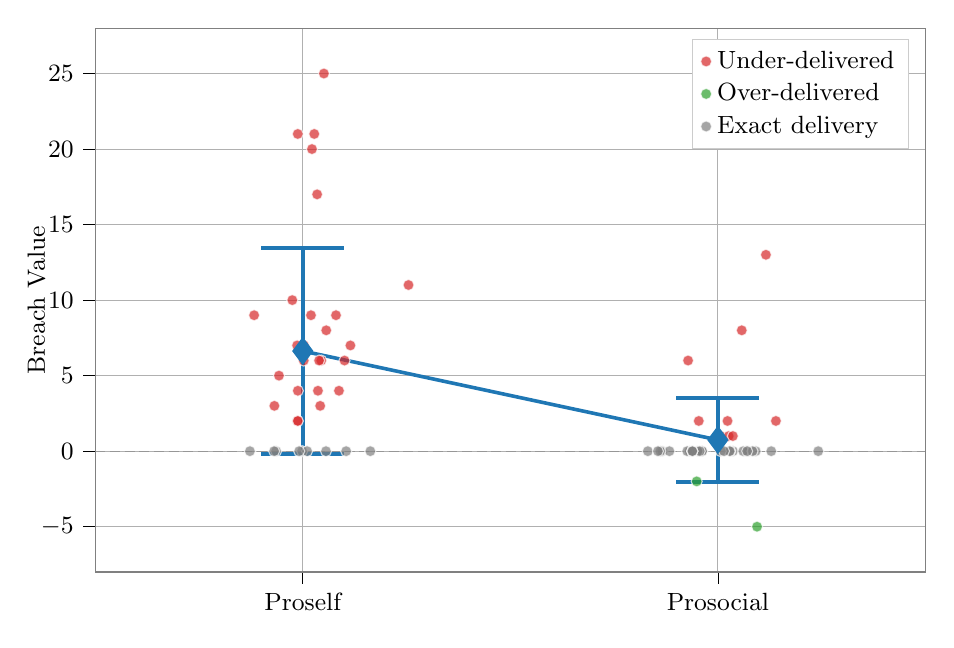
\begin{tikzpicture}[scale=1] % 整体缩放到原来的75%

\definecolor{crimson2143940}{RGB}{214,39,40}
\definecolor{darkgrey176}{RGB}{176,176,176}
\definecolor{forestgreen4416044}{RGB}{44,160,44}
\definecolor{grey}{RGB}{128,128,128}
\definecolor{grey127}{RGB}{127,127,127}
\definecolor{lightgrey204}{RGB}{204,204,204}
\definecolor{steelblue31119180}{RGB}{31,119,180}

\begin{axis}[
width=1\textwidth,    % 调整宽度
height=0.7\textwidth,   % 调整高度
axis line style={grey},
legend cell align={left},
legend style={
    fill opacity=1, 
    draw opacity=1, 
    text opacity=1, 
    draw=lightgrey204,
    font=\small        % 减小图例文字大小
},
tick align=outside,
tick pos=left,
tick label style={font=\small}, % 减小刻度标签文字大小
unbounded coords=jump,
x grid style={darkgrey176},
xmajorgrids,
xmin=-0.5, xmax=1.5,
xtick style={color=black},
xtick={0,1},
xticklabels={Proself,Prosocial},
y grid style={darkgrey176},
ylabel={Breach Value},
ylabel style={
    inner sep=0pt,    % 减少标签和轴的距离
    yshift=-5pt,
    font=\small% 微调标签位置
},
ymajorgrids,
ymin=-8, ymax=28,
ytick style={color=black}
]
\addplot [draw=white, fill=crimson2143940, mark=*, only marks, opacity=0.7]
table{%
x  y
0.0445638460840499 6
-0.0251492206481874 10
0.114781952236595 7
0.100617626838817 6
-0.0136131241983251 7
0.0872149291831909 4
-0.0572963889075815 5
-0.0118920383636059 4
-0.117137841801724 9
0.0509179870845854 25
0.0221982495680006 20
0.0346050065278643 17
0.00230769625747983 6
0.254731069003091 11
0.0393459215580669 6
-0.0120641631555385 21
0.0277365071623715 21
-0.0683417909118421 3
-0.0130147123380035 2
0.0420172585927707 3
-0.0118326818204489 2
0.0197717399460027 9
0.0800578994633806 9
0.0565739651290471 8
0.0365675958313638 4
0.00267953796925637 7
0.953947844949934 2
1.00659893512175 1
1.02599264664095 1
1.02320387746105 2
0.928213790904517 6
1.11573869264649 13
1.03610461954773 1
1.13981869672728 2
1.05748900969922 8
};
\addlegendentry{Under-delivered}
\addplot [draw=white, fill=forestgreen4416044, mark=*, only marks, opacity=0.7]
table{%
x  y
0.948996078943193 -2
1.09438747354748 -5
};
\addlegendentry{Over-delivered}
\addplot [draw=white, fill=grey127, mark=*, only marks, opacity=0.7]
table{%
x  y
-0.127308345407316 0
0.104520692071222 0
-0.0641762829563584 0
0.055957609290904 0
-0.0690108987612187 0
-0.00148865819560041 0
0.010467316369314 0
-0.00868031174757913 0
0.162803395945189 0
0.961671241805028 0
0.866342749234445 0
0.962145827755179 0
0.883295406035024 0
1.03623736893198 0
0.951216387630073 0
0.93821514743396 0
1.06768337023267 0
1.07418942436415 0
1.02972098441247 0
0.956204693829915 0
1.02844696233252 0
0.931802421814724 0
1.06119104521306 0
1.09106060861954 0
1.08352663180933 0
1.00699543775591 0
0.831289705831112 0
0.861294506495678 0
1.01475658604604 0
0.926218868506304 0
0.93826782575368 0
0.855588191755131 0
0.938356419492756 0
1.12858657125864 0
1.07049181342972 0
1.24179800517493 0
0.938632444210647 0
};
\addlegendentry{Exact delivery}
\addplot [line width=1.3pt, steelblue31119180, mark=diamond*, mark size=4.05, mark options={solid}, forget plot]
table {%
0 6.62857142857143
1 0.743589743589744
};
\addplot [line width=1.3pt, steelblue31119180, forget plot]
table {%
-0.1 -0.180098279475606
0.1 -0.180098279475606
nan nan
0 -0.180098279475606
0 13.4372411366185
nan nan
-0.1 13.4372411366185
0.1 13.4372411366185
};
\addplot [line width=1.3pt, steelblue31119180, forget plot]
table {%
0.9 -2.02577222661157
1.1 -2.02577222661157
nan nan
1 -2.02577222661157
1 3.51295171379106
nan nan
0.9 3.51295171379106
1.1 3.51295171379106
};
\addplot [grey, opacity=0.5, dash pattern=on 3.7pt off 1.6pt, forget plot]
table {%
-0.5 0
1.5 0
};
\end{axis}

\end{tikzpicture}
\caption{Contract breach patterns showing delivery deviations. }
\label{fig:svo_breach}
\end{subfigure}
\hfill
\begin{subfigure}[l]{0.48\textwidth}
\centering
% \includegraphics[width=\textwidth]{figs/svo_value.pdf}
% This file was created with tikzplotlib v0.10.1.
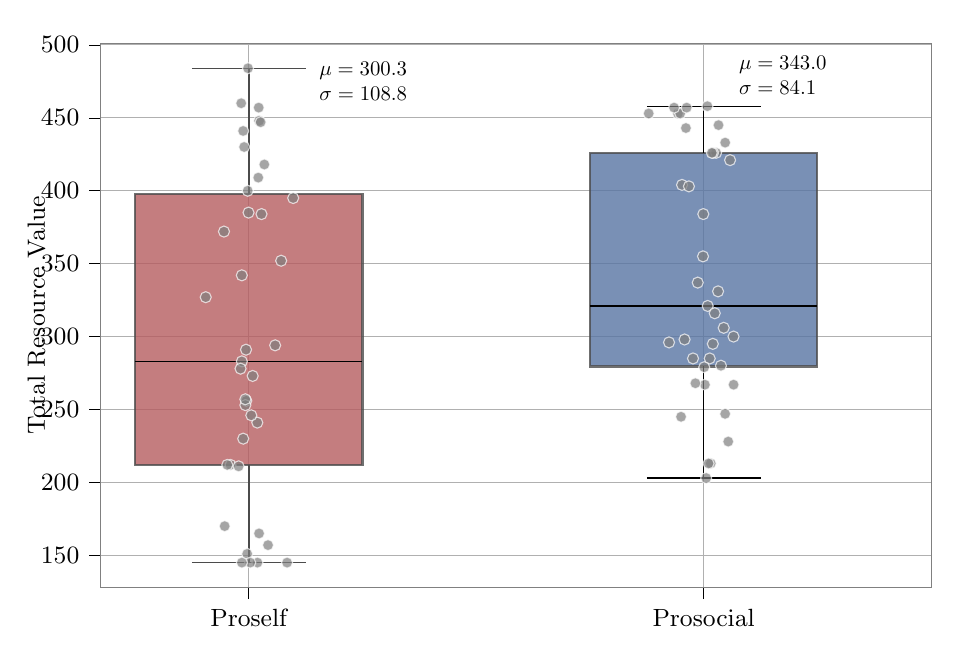
\begin{tikzpicture}[scale= 1]

\definecolor{darkgrey176}{RGB}{176,176,176}
\definecolor{darkslategrey}{RGB}{47,79,79}
\definecolor{darkslategrey75}{RGB}{75,75,75}
\definecolor{grey}{RGB}{128,128,128}
\definecolor{indianred1819295}{RGB}{181,92,95}
\definecolor{steelblue88116163}{RGB}{88,116,163}
\definecolor{grey127}{RGB}{127,127,127}
\begin{axis}[
    width=1\textwidth,    % 增加宽度
    height=0.7\textwidth,   % 保持高度
    axis line style={grey},
    legend cell align={left},
    legend style={
        fill opacity=1,
        draw opacity=1,
        text opacity=1,
        draw=lightgrey204,
        font=\small
    },
    tick align=outside,
    tick pos=left,
    tick label style={font=\small}, % 减小刻度标签文字大小
    unbounded coords=jump,
    x grid style={darkgrey176},
    xmajorgrids,
    xmin=-0.325,
    xmax=1.5,  % 增加右侧空间
    xtick style={color=black},
    xtick={0,1},
    xticklabels={Proself,Prosocial},
    y grid style={darkgrey176},
    ylabel={Total Resource Value},
    ylabel style={
        inner sep=0pt,    % 减少标签和轴的距离
        yshift=-5pt,
        font=\small% 微调标签位置
    },
    ymajorgrids,
    ymin=128.05,
    ymax=500.95,
    ytick style={color=black}
]

\path [draw=darkslategrey75, fill=indianred1819295, opacity=0.8, thick]
(axis cs:-0.25,212)
--(axis cs:0.25,212)
--(axis cs:0.25,397.5)
--(axis cs:-0.25,397.5)
--(axis cs:-0.25,212)
--cycle;
\addplot [thick, darkslategrey75]
table {%
0 212
0 145
};
\addplot [thick, darkslategrey75]
table {%
0 397.5
0 484
};
\addplot [darkslategrey75]
table {%
-0.125 145
0.125 145
};
\addplot [darkslategrey75]
table {%
-0.125 484
0.125 484
};
\path [draw=darkslategrey75, fill=steelblue88116163, opacity=0.8, thick]
(axis cs:0.75,279.5)
--(axis cs:1.25,279.5)
--(axis cs:1.25,426)
--(axis cs:0.75,426)
--(axis cs:0.75,279.5)
--cycle;
\addplot [semithick, black]
table {%
1 279.5
1 203
};
\addplot [semithick, black]
table {%
1 426
1 458
};
\addplot [black]
table {%
0.875 203
1.125 203
};
\addplot [black]
table {%
0.875 458
1.125 458
};
\addplot [semithick, black]
table {%
-0.25 283
0.25 283
};
\addplot [semithick, black]
table {%
0.75 321
1.25 321
};
\addplot [draw=white, fill=grey127, mark=*, only marks, opacity=0.7]
table{%
x  y
-0.0400714931851179 212
-0.0471077322208402 212
-0.00348859589556723 151
-0.00535089710335726 256
0.0188237301177679 241
-0.0528967007198037 170
0.0342792737565218 418
0.0227967510587223 448
0.021889248835996 457
0.0424060017506745 157
0.0226896689679356 165
0.0190811233108301 145
0.0842751337063159 145
0.00328385078573139 145
-0.015058423667463 145
-0.00225422671150385 400
-0.0151309330843346 283
0.0580573976352849 294
-0.007403861239717 253
-0.00746582744592909 257
-0.0222577633297763 211
-0.0945623517165704 327
-0.000459986797348707 385
0.0260911422409645 447
-0.054421902227173 372
0.0209726357676193 409
0.0280668742631608 384
-0.015211997737578 342
0.0977132767945952 395
-0.012148787362295 230
-0.018010351217818 278
0.00865172163974299 273
0.00561699758303698 246
-0.0165485111999984 460
-0.0100909696563266 430
-0.0122865212285328 441
-0.00598001510483728 291
0.0712729100178481 352
-0.001671465968594 484
};
\addplot [draw=white, fill=grey127, mark=*, only marks, opacity=0.7]
table{%
x  y
1.0441367553066 306
1.0027332433394 267
0.95806292071245 298
0.950327774587431 245
0.976652722074529 285
1.01329328712134 285
1.06579537883704 267
1.01558799679811 213
1.00554778845784 203
0.981861072208001 268
1.03799438299505 280
1.00887494972378 321
1.06565853282715 300
1.02432677880316 316
0.986987431934729 337
1.05404842765952 228
0.923907194855337 296
1.00122851638026 279
1.01072624258051 213
1.02014635388555 295
1.03169376989667 331
0.943346312961445 453
0.87918469572047 453
0.948499504536591 453
1.02738130216741 426
1.02066958997992 426
1.05808479915307 421
1.01797718789997 426
0.960991304116238 443
1.00825805416717 458
1.04721016525747 247
0.998592361718987 355
1.03265007319596 445
1.04729862844036 433
0.999219551792941 384
0.952445320354032 404
0.967587585006039 403
0.96264876180953 457
0.934955276115197 457
};

% 调整统计信息的位置和样式
\draw (axis cs:0.15,490) node[
  scale=0.75,
  fill=none,
  draw=none,
  inner sep=1pt,
  anchor=north west,
  text=black,
  align=left
]{\bfseries $\mu = 300.3$\\
$\sigma = 108.8$};

\draw (axis cs:1.07,495) node[
  scale=0.75,
  fill=none,
  draw=none,
  inner sep=1.5pt,
  anchor=north west,
  text=black,
  align=left
]{\bfseries $\mu = 343.0$\\
$\sigma = 84.1$};

\end{axis}
\end{tikzpicture}
\caption{Distribution of agent total resource values.}
\label{fig:svo_value}
\end{subfigure}
\caption{Behavioral comparison between Proself and Prosocial agents.}
\label{fig:svo_comparison}
\end{figure*}

In this section, we are curious about the influence of social value orientations on human exchange behaviors.
Specifically, we conduct experiments by setting the agents to be Proself and Prosocial, respectively, and then collect their behaviors for analysis.
% The SVO framework in our agent society provides a lens to examine how individual preferences between self-interest and mutual benefit affect exchange dynamics. Our experiments compare Proself and Prosocial agents across ten trials for each group.
% , incorporating both Rational and Experiential cognitive profiles to ensure comprehensive behavioral analysis.
Figure~\ref{fig:svo_comparison} reveals behavioral differences between the two orientations. We can see, Proself agents exhibit significantly higher rates of strategic breaching, predominantly through under-delivery of promised resources. This pattern reflects their prioritization of immediate personal gains over contractual commitments. In contrast, Prosocial agents demonstrate notably higher fidelity to exchange agreements, with most data points clustering around exact delivery.
The economic consequences of these behavioral differences, illustrated in Figure~\ref{fig:svo_value}, reveal significant differences. While Proself agents show wider outcome variability ($\mu$ = 300.3, $\sigma$ = 108.8) and occasionally achieve higher individual values, their exchange patterns result in lower average outcomes. Prosocial agents achieve higher mean values ($\mu$ = 343.0, $\sigma$ = 84.1) with more consistent distributions, suggesting that maintaining stable exchange relationships benefits long-term value accumulation.

These observations lead us to propose the second corollary of Homans' SET:
\begin{corollary}[The Reciprocity Corollary]
% In social exchange systems, behaviors optimizing collective interests generate higher aggregate value than those maximizing individual gains, though they may constrain individual peak performance.
Exchange behaviors guided by mutual benefit principles lead to more stable and efficient resource distribution in social exchange systems.
\end{corollary}
This corollary extends our understanding of social exchange dynamics by highlighting the complex interplay between individual and reciprocal optimization. Although Proself strategies may optimize individual outcomes in specific scenarios, Prosocial orientations consistently generate more robust and efficient exchange networks. 

% Empirical evidence demonstrates that choosing between these orientations presents a fundamental tradeoff between maximizing individual potential and achieving optimal system-level efficiency.



\subsection{Social System Resilience}

Building upon the case study shown in Figure~\ref{fig:case}, we extended our simulation for an additional ten rounds to examine system behavior after significant trust violations. Figure~\ref{fig:case_20r} illustrates the exchange dynamics across this extended period. The data reveals that while agents initially reduce their exchange activity following trust breaches, they gradually resume exchanges through adaptive strategies. The patterns show that while Agent C maintains relatively stable exchange value, Agent A and Agent B exhibit more volatile behaviors. The persistent exchange patterns between rounds 10-20 suggest an inherent system stability driven by fundamental exchange need of each agent.

Based on these observations, we have the third corollary of Homans' SET:
\begin{corollary}[The Resilience Corollary]
% In multi-agent exchange systems, market-like mechanisms emerge from individual rational choices, creating self-stabilizing patterns that maintain system functionality and value creation despite periodic disruptions.
% In multi-agent exchange systems, periodic disruptions trigger compensatory behaviors that restore system functionality through self-organizing exchange patterns, maintaining sustainable trading activities within stable bounds.
% When disrupted, a social exchange system will return to stability through self-organizing behaviors of its members, where stability manifests as sustained trading activities within fluctuating bounds.
% An established social exchange system naturally regains stability through member adaptation.
An established social exchange system tends toward stability through member adaptation, driven by their interdependent resource needs.
\end{corollary}

The above three corollaries extend Homans' SET by highlighting the complex interplay between cognitive processing style, individual orientation, and system-level resilience. Together, they provide new insights into the mechanisms that govern social exchange systems, whether human or artificial.


\subsection{Real-World Experiments on Evaluating the Corollaries of Homans' SET}
In this section, we aim to empirically evaluate the corollaries proposed above with real human experiments.
Since it is quite difficult to control real human cognitive styles and social value orientations, we focus on the resilience corollary.

In specific, 
% we conducted comparative experiments between human participants and LLM agents. 
we recruited three human participants, 
% and measured their dispositional and cognitive characteristics through SVO and REI assessments. 
and let each of them interact with two LLM-based agents in the constructed agent society. These agents are programmed to violate trust at round 10 by withholding all previously promised resources. 
For comparison, we conducted parallel agent trials, in which each human participant was replaced by an LLM agent under the same conditions.
The detailed procedure of human experiments is described in Appendix~\ref{sec:human}.


As illustrated in Figure~\ref{fig:system}, the observed exchange patterns in both human and agent trials demonstrate remarkable similarities. Despite the trust violations by the controlled agents, both humans and agents continue exchange and gradually reach a stable state with fluctuating but persistent exchange levels. These consistent patterns validate our resilience corollary while demonstrating that our agent framework effectively captures how people adapt to trust violations in social exchanges. 

% Through this parallel experimentation between humans and agents, we extend SET by revealing social exchange systems' self-stabilizing properties and provide empirical support for the Resilience Corollary.

% As shown in Figure~\ref{fig:system}, the trading patterns in both human and agent trials demonstrate remarkable similarities, validating our corollary. Despite the trust violations by the controlled agents, both humans and agents continue trading and gradually reach a stable state with fluctuating but persistent trading levels. The similar patterns between human and agent behaviors demonstrate that our agent-based simulation effectively captures how people adapt to trust violations in social exchanges.


% This corollary extends SET by revealing social exchange systems' self-stabilizing properties. The remarkable similarity between human and agent exchange patterns validates that our agent framework effectively captures human behavioral patterns in response to trust violations. Through parallel experiments, we demonstrate how exchange systems achieve dynamic equilibrium through adaptive behaviors, providing empirical support for the Resilience Corollary.

% This corollary extends SET by revealing how exchange systems naturally stabilize after trust violations. Our experiments with both human and agent participants demonstrate that such systems achieve dynamic equilibrium through adaptive behaviors.
%aligning with Gode and Sunder's ~\cite{gode1993allocative} findings on emergent stability patterns.

% This corollary extends our understanding of social exchange dynamics by revealing how established social exchange systems exhibit inherent resilience following trust violations. The convergent findings from both human and agent experiments demonstrate that social exchange systems can maintain stability even after severe trust violations, achieving dynamic equilibrium through adaptive behaviors. This finding extends Homans' SET with new insights about system resilience, and resonates with Gode and Sunder ~\cite{gode1993allocative} on stable pattern emergence in exchange systems.



% To validate this corollary, we conducted experiments with three human participants each interacting with two LLM agents (Alice and Bob) configured with proself and rational profiles. At round 10, the agents were programmed to breach trust by withholding all promised resources. As shown in Figure~\ref{fig:human}, the trading patterns validate our corollary: despite the trust violation, the system maintains trading activities and reaches a new stable state. However, humans exhibit a more conservative recovery compared to purely rational agents, with trading volumes stabilizing at a lower level. This difference can be attributed to the emotional impact of betrayal on human participants, who, unlike rational agents, factor emotional responses into their decision-making and adopt more cautious strategies to protect against future violations.





% This corollary extends our understanding of social exchange dynamics by revealing the inherent resilience of social exchange systems. The convergent findings from both agent simulations and human experiments align with Gode and Sunder's theory ~\cite{gode1993allocative} that stable trading patterns naturally emerge in exchange systems, while also highlighting the robustness of these patterns across both artificial and human social systems.





\begin{figure}[t]
\centering
\begin{subfigure}[r]{0.5\textwidth}
\centering
% \includegraphics[width=\textwidth]{figs/svo_breach.pdf}
% This file was created with tikzplotlib v0.10.1.
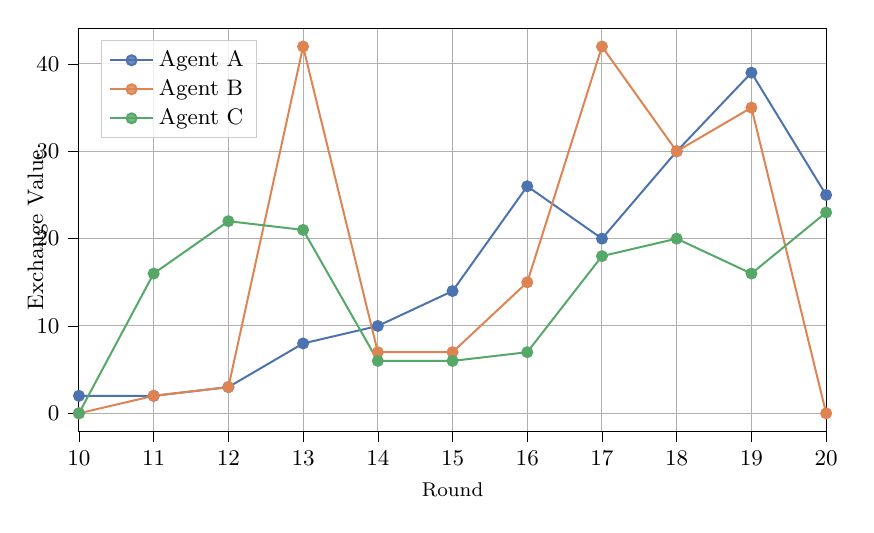
\begin{tikzpicture}[scale=0.9]
\definecolor{darkgrey176}{RGB}{176,176,176}
\definecolor{darkorange25512714}{RGB}{221,132,82}
\definecolor{forestgreen4416044}{RGB}{85,168,104}
\definecolor{lightgrey204}{RGB}{204,204,204}
\definecolor{steelblue31119180}{RGB}{76,114,176}
\begin{axis}[
scale=1,           
width=1\textwidth,  % 减半宽度
height=0.6\textwidth,
legend cell align={left},
legend style={
  fill opacity=0.8,
  draw opacity=1,
  text opacity=1,
  at={(0.03,0.97)},
  anchor=north west,
  draw=lightgrey204,
  font=\small
},
tick align=outside,
tick pos=left,
x grid style={darkgrey176},
tick label style={font=\small},
xmajorgrids,
xmin=10, xmax=20,    % 保持原始坐标范围
xtick style={color=black},
y grid style={darkgrey176},
xlabel=Round,
xlabel style={font=\footnotesize},
ylabel={Exchange Value},
ylabel style={
    inner sep=0pt,    
    yshift=-8pt,
    font=\small
},
ymajorgrids,
ymin=-2.1, ymax=44.1,
ytick style={color=black}
]
\addplot [thick, steelblue31119180, mark=*, mark size=2, mark options={solid}]
table {%
10 2
11 2
12 3
13 8
14 10
15 14
16 26
17 20
18 30
19 39
20 25
};
\addlegendentry{Agent A}
\addplot [thick, darkorange25512714, mark=*, mark size=2, mark options={solid}]
table {%
10 0
11 2
12 3
13 42
14 7
15 7
16 15
17 42
18 30
19 35
20 0
};
\addlegendentry{Agent B}
\addplot [thick, forestgreen4416044, mark=*, mark size=2, mark options={solid}]
table {%
10 0
11 16
12 22
13 21
14 6
15 6
16 7
17 18
18 20
19 16
20 23
};
\addlegendentry{Agent C}
\end{axis}
\end{tikzpicture}
\caption{Per-round exchange values between three agents. }
\label{fig:case_20r}
\end{subfigure}
\hfill
\begin{subfigure}[l]{0.5\textwidth}
\centering
% \includegraphics[width=\textwidth]{figs/svo_value.pdf}
\begin{figure}
    \centering
    \begin{subfigure}[t]{0.465\columnwidth}
    \centering
    \includegraphics[width=\textwidth, trim=15 15 15 0, clip]{Images/Experiments/distance_to_front_manual_test_together.pdf}
    \caption{Human driving behavior for scenario 1 illustrated by the distance to the front vehicle}.
    \label{fig:human}
    \end{subfigure} \hfill
    \begin{subfigure}[t]{0.465\columnwidth}
    \centering
        \includegraphics[width=\textwidth, trim=25 0 0 0, clip]{Images/Experiments/example_trip.png}
        \caption{Agent's driving behavior during one random sampled episode in MPC case trained in experiment 3.}
        \label{fig:example}
    \end{subfigure}
    \caption{Left: Human driving behavior in our simulator settings. Right: An example of the agent's driving behavior during the MPC case with fixed time steps for switching the case.}
\end{figure}
\caption{Comparison of exchange values between humans and agents.}
\label{fig:human}
\end{subfigure}
\caption{Exchange dynamics following trust violations. }
\label{fig:system}
\end{figure}



% \subsection{Influence of Initial Affinity}

\section{Related Work}

\subsection{Homans Social Exchange Theory}
% Social Exchange Theory (SET) is a foundational framework in sociology and social psychology that views social interactions as transactions of value~\cite{homans1958social}. SET has been widely applied to explain organizational behavior, leadership trust, and workplace relationships~\cite{ahmad2023social}, while also illuminating friendships~\cite{methot2016workplace}, family relations~\cite{cropanzano2005social}, and romantic partnerships~\cite{laursen1999nature}. Recent theoretical advances include Lawler and Thye's~\cite{lawler2006social} exploration of emotional dimensions and Cropanzano et al.'s~\cite{cropanzano2017social} two-dimensional model incorporating activity alongside hedonic factors. While Enayat et al.~\cite{enayat2022computational} implemented SET through multi-agent simulation, their simplified exchange rules overlooked emotional complexity. Our approach leverages LLM-driven agents to simulate more nuanced human interactions, offering a more faithful implementation of SET.
Social Exchange Theory is a foundational framework in sociology and social psychology that views social interactions as transactions of value~\cite{homans1958social}. In organizational and workplace behavior, it is considered a “gold standard” for explaining dynamics like employee–employer relationships, leadership trust, and organizational citizenship behaviors~\cite{ahmad2023social}. Beyond organizations, SET has been used in social psychology to examine friendships~\cite{methot2016workplace}, family relations~\cite{cropanzano2005social}, and even romantic partnerships~\cite{laursen1999nature} as exchanges of emotional support, information, and other resources. 

Recent refinements to SET have deepened its explanatory power. Lawler and Thye~\cite{lawler2006social} explored the emotional dimensions of exchange, while Cropanzano et al.\cite{cropanzano2017social} proposed a two-dimensional model incorporating "activity" alongside the traditional hedonic framework, enhancing SET’s predictive accuracy. In terms of research methods, Enayat et al.\cite{enayat2022computational} applied SET in a multi-agent simulation to explore social structures through simplified exchange rules. However, their model, which reduced agent behavior to simple exchanges of money and recognition, overlooked emotional subjectivity. To address this limitation, our approach employs LLM-driven agents to simulate more complex human interactions, offering a more accurate implementation of SET.

 
\subsection{LLM-driven Agent-based Modeling}

% LLMs have transformed agent-based modeling by enabling human-like behavior and decision-making capabilities~\cite{gao2024large}. Key developments include Generative Agent~\cite{park2023generative}, which simulates community life with 25 LLM agents, EconAgent~\cite{li2024econagent}, which explores macroeconomic phenomena, and RecAgent~\cite{wang2023user}, which studies recommender system interactions. Recent works have demonstrated LLM agents' ability to simulate classical social scenarios, with CompeteAI~\cite{zhao2023competeai} modeling competitive behavior and Xie et al.~\cite{xie2024can} exploring trust dynamics. Building on these advances, our work presents a novel application of LLM-driven agents to validate and extend SET.

The rise of LLMs has significantly advanced agent-based modeling by enabling agents with human-like behavior and decision-making capabilities. Traditionally, ABM relied on fixed rules to govern agent behavior, but LLMs provide flexible, dynamic responses that better simulate real human interactions~\cite{gao2024large}. Several studies have leveraged LLMs to enhance ABM across different domains. Generative Agent\cite{park2023generative}, which simulates daily life in a virtual town with 25 LLM agents, and EconAgent\cite{li2024econagent}, a model that uses LLM agents to explore macroeconomic phenomena. RecAgent~\cite{wang2023user} studies user interaction with recommender systems through LLM-driven agents.

LLM agents have also been used to simulate classical social scenarios, such as competition and trust. CompeteAI\cite{zhao2023competeai} models competitive behavior between restaurant owners, while Xie et al.\cite{xie2024can} explore trust dynamics in LLM agents. These studies demonstrate LLM agents' ability to replicate human-like patterns of social behavior. Building on this, our work aims to validate and extend SET using LLM-driven agent-based modeling, a domain that has yet to be extensively explored in the context of SET.


\section{Conclusion}
In this paper, we demonstrated that LLM agents can effectively replicate and help study human social exchange behaviors. Through our structured experimental framework, we validated Homans' SET propositions and proposed new corollaries that extend our understanding of social exchange dynamics in multi-agent systems. While our controlled environment and simplified resource exchange scenario may not fully capture the complexity of real-world social interactions, the consistent behavioral patterns observed across different agent profiles suggest promising directions for future research. Further studies could explore more complex exchange scenarios, investigate the impact of environmental variables, and conduct comparative analyses between LLM agents and human subjects to validate the generalizability of our findings.


\section*{Limitations}
There are several limitations of this paper. First, our experimental environment is relatively simplified, with structured negotiation protocols and basic resource types that may not fully capture the complexity of real-world social exchanges. Second, due to LLM API cost constraints, we were limited in the number of experimental trials and rounds, which may affect the generalizability of our findings. Third, while agents provide rationales for their decisions, our analysis of their internal thought processes and detailed exchange behaviors could be more comprehensive. Finally, we did not consider the potential impact of cultural factors on exchange dynamics. Future research could address these limitations by designing more complex exchange scenarios, conducting larger-scale experiments, performing deeper analysis of agent decision processes, and examining the role of cultural variations in social exchanges.

% Bibliography entries for the entire Anthology, followed by custom entries
%\bibliography{anthology,custom}
% Custom bibliography entries only
\bibliography{custom}

\appendix

\subsection{Lloyd-Max Algorithm}
\label{subsec:Lloyd-Max}
For a given quantization bitwidth $B$ and an operand $\bm{X}$, the Lloyd-Max algorithm finds $2^B$ quantization levels $\{\hat{x}_i\}_{i=1}^{2^B}$ such that quantizing $\bm{X}$ by rounding each scalar in $\bm{X}$ to the nearest quantization level minimizes the quantization MSE. 

The algorithm starts with an initial guess of quantization levels and then iteratively computes quantization thresholds $\{\tau_i\}_{i=1}^{2^B-1}$ and updates quantization levels $\{\hat{x}_i\}_{i=1}^{2^B}$. Specifically, at iteration $n$, thresholds are set to the midpoints of the previous iteration's levels:
\begin{align*}
    \tau_i^{(n)}=\frac{\hat{x}_i^{(n-1)}+\hat{x}_{i+1}^{(n-1)}}2 \text{ for } i=1\ldots 2^B-1
\end{align*}
Subsequently, the quantization levels are re-computed as conditional means of the data regions defined by the new thresholds:
\begin{align*}
    \hat{x}_i^{(n)}=\mathbb{E}\left[ \bm{X} \big| \bm{X}\in [\tau_{i-1}^{(n)},\tau_i^{(n)}] \right] \text{ for } i=1\ldots 2^B
\end{align*}
where to satisfy boundary conditions we have $\tau_0=-\infty$ and $\tau_{2^B}=\infty$. The algorithm iterates the above steps until convergence.

Figure \ref{fig:lm_quant} compares the quantization levels of a $7$-bit floating point (E3M3) quantizer (left) to a $7$-bit Lloyd-Max quantizer (right) when quantizing a layer of weights from the GPT3-126M model at a per-tensor granularity. As shown, the Lloyd-Max quantizer achieves substantially lower quantization MSE. Further, Table \ref{tab:FP7_vs_LM7} shows the superior perplexity achieved by Lloyd-Max quantizers for bitwidths of $7$, $6$ and $5$. The difference between the quantizers is clear at 5 bits, where per-tensor FP quantization incurs a drastic and unacceptable increase in perplexity, while Lloyd-Max quantization incurs a much smaller increase. Nevertheless, we note that even the optimal Lloyd-Max quantizer incurs a notable ($\sim 1.5$) increase in perplexity due to the coarse granularity of quantization. 

\begin{figure}[h]
  \centering
  \includegraphics[width=0.7\linewidth]{sections/figures/LM7_FP7.pdf}
  \caption{\small Quantization levels and the corresponding quantization MSE of Floating Point (left) vs Lloyd-Max (right) Quantizers for a layer of weights in the GPT3-126M model.}
  \label{fig:lm_quant}
\end{figure}

\begin{table}[h]\scriptsize
\begin{center}
\caption{\label{tab:FP7_vs_LM7} \small Comparing perplexity (lower is better) achieved by floating point quantizers and Lloyd-Max quantizers on a GPT3-126M model for the Wikitext-103 dataset.}
\begin{tabular}{c|cc|c}
\hline
 \multirow{2}{*}{\textbf{Bitwidth}} & \multicolumn{2}{|c|}{\textbf{Floating-Point Quantizer}} & \textbf{Lloyd-Max Quantizer} \\
 & Best Format & Wikitext-103 Perplexity & Wikitext-103 Perplexity \\
\hline
7 & E3M3 & 18.32 & 18.27 \\
6 & E3M2 & 19.07 & 18.51 \\
5 & E4M0 & 43.89 & 19.71 \\
\hline
\end{tabular}
\end{center}
\end{table}

\subsection{Proof of Local Optimality of LO-BCQ}
\label{subsec:lobcq_opt_proof}
For a given block $\bm{b}_j$, the quantization MSE during LO-BCQ can be empirically evaluated as $\frac{1}{L_b}\lVert \bm{b}_j- \bm{\hat{b}}_j\rVert^2_2$ where $\bm{\hat{b}}_j$ is computed from equation (\ref{eq:clustered_quantization_definition}) as $C_{f(\bm{b}_j)}(\bm{b}_j)$. Further, for a given block cluster $\mathcal{B}_i$, we compute the quantization MSE as $\frac{1}{|\mathcal{B}_{i}|}\sum_{\bm{b} \in \mathcal{B}_{i}} \frac{1}{L_b}\lVert \bm{b}- C_i^{(n)}(\bm{b})\rVert^2_2$. Therefore, at the end of iteration $n$, we evaluate the overall quantization MSE $J^{(n)}$ for a given operand $\bm{X}$ composed of $N_c$ block clusters as:
\begin{align*}
    \label{eq:mse_iter_n}
    J^{(n)} = \frac{1}{N_c} \sum_{i=1}^{N_c} \frac{1}{|\mathcal{B}_{i}^{(n)}|}\sum_{\bm{v} \in \mathcal{B}_{i}^{(n)}} \frac{1}{L_b}\lVert \bm{b}- B_i^{(n)}(\bm{b})\rVert^2_2
\end{align*}

At the end of iteration $n$, the codebooks are updated from $\mathcal{C}^{(n-1)}$ to $\mathcal{C}^{(n)}$. However, the mapping of a given vector $\bm{b}_j$ to quantizers $\mathcal{C}^{(n)}$ remains as  $f^{(n)}(\bm{b}_j)$. At the next iteration, during the vector clustering step, $f^{(n+1)}(\bm{b}_j)$ finds new mapping of $\bm{b}_j$ to updated codebooks $\mathcal{C}^{(n)}$ such that the quantization MSE over the candidate codebooks is minimized. Therefore, we obtain the following result for $\bm{b}_j$:
\begin{align*}
\frac{1}{L_b}\lVert \bm{b}_j - C_{f^{(n+1)}(\bm{b}_j)}^{(n)}(\bm{b}_j)\rVert^2_2 \le \frac{1}{L_b}\lVert \bm{b}_j - C_{f^{(n)}(\bm{b}_j)}^{(n)}(\bm{b}_j)\rVert^2_2
\end{align*}

That is, quantizing $\bm{b}_j$ at the end of the block clustering step of iteration $n+1$ results in lower quantization MSE compared to quantizing at the end of iteration $n$. Since this is true for all $\bm{b} \in \bm{X}$, we assert the following:
\begin{equation}
\begin{split}
\label{eq:mse_ineq_1}
    \tilde{J}^{(n+1)} &= \frac{1}{N_c} \sum_{i=1}^{N_c} \frac{1}{|\mathcal{B}_{i}^{(n+1)}|}\sum_{\bm{b} \in \mathcal{B}_{i}^{(n+1)}} \frac{1}{L_b}\lVert \bm{b} - C_i^{(n)}(b)\rVert^2_2 \le J^{(n)}
\end{split}
\end{equation}
where $\tilde{J}^{(n+1)}$ is the the quantization MSE after the vector clustering step at iteration $n+1$.

Next, during the codebook update step (\ref{eq:quantizers_update}) at iteration $n+1$, the per-cluster codebooks $\mathcal{C}^{(n)}$ are updated to $\mathcal{C}^{(n+1)}$ by invoking the Lloyd-Max algorithm \citep{Lloyd}. We know that for any given value distribution, the Lloyd-Max algorithm minimizes the quantization MSE. Therefore, for a given vector cluster $\mathcal{B}_i$ we obtain the following result:

\begin{equation}
    \frac{1}{|\mathcal{B}_{i}^{(n+1)}|}\sum_{\bm{b} \in \mathcal{B}_{i}^{(n+1)}} \frac{1}{L_b}\lVert \bm{b}- C_i^{(n+1)}(\bm{b})\rVert^2_2 \le \frac{1}{|\mathcal{B}_{i}^{(n+1)}|}\sum_{\bm{b} \in \mathcal{B}_{i}^{(n+1)}} \frac{1}{L_b}\lVert \bm{b}- C_i^{(n)}(\bm{b})\rVert^2_2
\end{equation}

The above equation states that quantizing the given block cluster $\mathcal{B}_i$ after updating the associated codebook from $C_i^{(n)}$ to $C_i^{(n+1)}$ results in lower quantization MSE. Since this is true for all the block clusters, we derive the following result: 
\begin{equation}
\begin{split}
\label{eq:mse_ineq_2}
     J^{(n+1)} &= \frac{1}{N_c} \sum_{i=1}^{N_c} \frac{1}{|\mathcal{B}_{i}^{(n+1)}|}\sum_{\bm{b} \in \mathcal{B}_{i}^{(n+1)}} \frac{1}{L_b}\lVert \bm{b}- C_i^{(n+1)}(\bm{b})\rVert^2_2  \le \tilde{J}^{(n+1)}   
\end{split}
\end{equation}

Following (\ref{eq:mse_ineq_1}) and (\ref{eq:mse_ineq_2}), we find that the quantization MSE is non-increasing for each iteration, that is, $J^{(1)} \ge J^{(2)} \ge J^{(3)} \ge \ldots \ge J^{(M)}$ where $M$ is the maximum number of iterations. 
%Therefore, we can say that if the algorithm converges, then it must be that it has converged to a local minimum. 
\hfill $\blacksquare$


\begin{figure}
    \begin{center}
    \includegraphics[width=0.5\textwidth]{sections//figures/mse_vs_iter.pdf}
    \end{center}
    \caption{\small NMSE vs iterations during LO-BCQ compared to other block quantization proposals}
    \label{fig:nmse_vs_iter}
\end{figure}

Figure \ref{fig:nmse_vs_iter} shows the empirical convergence of LO-BCQ across several block lengths and number of codebooks. Also, the MSE achieved by LO-BCQ is compared to baselines such as MXFP and VSQ. As shown, LO-BCQ converges to a lower MSE than the baselines. Further, we achieve better convergence for larger number of codebooks ($N_c$) and for a smaller block length ($L_b$), both of which increase the bitwidth of BCQ (see Eq \ref{eq:bitwidth_bcq}).


\subsection{Additional Accuracy Results}
%Table \ref{tab:lobcq_config} lists the various LOBCQ configurations and their corresponding bitwidths.
\begin{table}
\setlength{\tabcolsep}{4.75pt}
\begin{center}
\caption{\label{tab:lobcq_config} Various LO-BCQ configurations and their bitwidths.}
\begin{tabular}{|c||c|c|c|c||c|c||c|} 
\hline
 & \multicolumn{4}{|c||}{$L_b=8$} & \multicolumn{2}{|c||}{$L_b=4$} & $L_b=2$ \\
 \hline
 \backslashbox{$L_A$\kern-1em}{\kern-1em$N_c$} & 2 & 4 & 8 & 16 & 2 & 4 & 2 \\
 \hline
 64 & 4.25 & 4.375 & 4.5 & 4.625 & 4.375 & 4.625 & 4.625\\
 \hline
 32 & 4.375 & 4.5 & 4.625& 4.75 & 4.5 & 4.75 & 4.75 \\
 \hline
 16 & 4.625 & 4.75& 4.875 & 5 & 4.75 & 5 & 5 \\
 \hline
\end{tabular}
\end{center}
\end{table}

%\subsection{Perplexity achieved by various LO-BCQ configurations on Wikitext-103 dataset}

\begin{table} \centering
\begin{tabular}{|c||c|c|c|c||c|c||c|} 
\hline
 $L_b \rightarrow$& \multicolumn{4}{c||}{8} & \multicolumn{2}{c||}{4} & 2\\
 \hline
 \backslashbox{$L_A$\kern-1em}{\kern-1em$N_c$} & 2 & 4 & 8 & 16 & 2 & 4 & 2  \\
 %$N_c \rightarrow$ & 2 & 4 & 8 & 16 & 2 & 4 & 2 \\
 \hline
 \hline
 \multicolumn{8}{c}{GPT3-1.3B (FP32 PPL = 9.98)} \\ 
 \hline
 \hline
 64 & 10.40 & 10.23 & 10.17 & 10.15 &  10.28 & 10.18 & 10.19 \\
 \hline
 32 & 10.25 & 10.20 & 10.15 & 10.12 &  10.23 & 10.17 & 10.17 \\
 \hline
 16 & 10.22 & 10.16 & 10.10 & 10.09 &  10.21 & 10.14 & 10.16 \\
 \hline
  \hline
 \multicolumn{8}{c}{GPT3-8B (FP32 PPL = 7.38)} \\ 
 \hline
 \hline
 64 & 7.61 & 7.52 & 7.48 &  7.47 &  7.55 &  7.49 & 7.50 \\
 \hline
 32 & 7.52 & 7.50 & 7.46 &  7.45 &  7.52 &  7.48 & 7.48  \\
 \hline
 16 & 7.51 & 7.48 & 7.44 &  7.44 &  7.51 &  7.49 & 7.47  \\
 \hline
\end{tabular}
\caption{\label{tab:ppl_gpt3_abalation} Wikitext-103 perplexity across GPT3-1.3B and 8B models.}
\end{table}

\begin{table} \centering
\begin{tabular}{|c||c|c|c|c||} 
\hline
 $L_b \rightarrow$& \multicolumn{4}{c||}{8}\\
 \hline
 \backslashbox{$L_A$\kern-1em}{\kern-1em$N_c$} & 2 & 4 & 8 & 16 \\
 %$N_c \rightarrow$ & 2 & 4 & 8 & 16 & 2 & 4 & 2 \\
 \hline
 \hline
 \multicolumn{5}{|c|}{Llama2-7B (FP32 PPL = 5.06)} \\ 
 \hline
 \hline
 64 & 5.31 & 5.26 & 5.19 & 5.18  \\
 \hline
 32 & 5.23 & 5.25 & 5.18 & 5.15  \\
 \hline
 16 & 5.23 & 5.19 & 5.16 & 5.14  \\
 \hline
 \multicolumn{5}{|c|}{Nemotron4-15B (FP32 PPL = 5.87)} \\ 
 \hline
 \hline
 64  & 6.3 & 6.20 & 6.13 & 6.08  \\
 \hline
 32  & 6.24 & 6.12 & 6.07 & 6.03  \\
 \hline
 16  & 6.12 & 6.14 & 6.04 & 6.02  \\
 \hline
 \multicolumn{5}{|c|}{Nemotron4-340B (FP32 PPL = 3.48)} \\ 
 \hline
 \hline
 64 & 3.67 & 3.62 & 3.60 & 3.59 \\
 \hline
 32 & 3.63 & 3.61 & 3.59 & 3.56 \\
 \hline
 16 & 3.61 & 3.58 & 3.57 & 3.55 \\
 \hline
\end{tabular}
\caption{\label{tab:ppl_llama7B_nemo15B} Wikitext-103 perplexity compared to FP32 baseline in Llama2-7B and Nemotron4-15B, 340B models}
\end{table}

%\subsection{Perplexity achieved by various LO-BCQ configurations on MMLU dataset}


\begin{table} \centering
\begin{tabular}{|c||c|c|c|c||c|c|c|c|} 
\hline
 $L_b \rightarrow$& \multicolumn{4}{c||}{8} & \multicolumn{4}{c||}{8}\\
 \hline
 \backslashbox{$L_A$\kern-1em}{\kern-1em$N_c$} & 2 & 4 & 8 & 16 & 2 & 4 & 8 & 16  \\
 %$N_c \rightarrow$ & 2 & 4 & 8 & 16 & 2 & 4 & 2 \\
 \hline
 \hline
 \multicolumn{5}{|c|}{Llama2-7B (FP32 Accuracy = 45.8\%)} & \multicolumn{4}{|c|}{Llama2-70B (FP32 Accuracy = 69.12\%)} \\ 
 \hline
 \hline
 64 & 43.9 & 43.4 & 43.9 & 44.9 & 68.07 & 68.27 & 68.17 & 68.75 \\
 \hline
 32 & 44.5 & 43.8 & 44.9 & 44.5 & 68.37 & 68.51 & 68.35 & 68.27  \\
 \hline
 16 & 43.9 & 42.7 & 44.9 & 45 & 68.12 & 68.77 & 68.31 & 68.59  \\
 \hline
 \hline
 \multicolumn{5}{|c|}{GPT3-22B (FP32 Accuracy = 38.75\%)} & \multicolumn{4}{|c|}{Nemotron4-15B (FP32 Accuracy = 64.3\%)} \\ 
 \hline
 \hline
 64 & 36.71 & 38.85 & 38.13 & 38.92 & 63.17 & 62.36 & 63.72 & 64.09 \\
 \hline
 32 & 37.95 & 38.69 & 39.45 & 38.34 & 64.05 & 62.30 & 63.8 & 64.33  \\
 \hline
 16 & 38.88 & 38.80 & 38.31 & 38.92 & 63.22 & 63.51 & 63.93 & 64.43  \\
 \hline
\end{tabular}
\caption{\label{tab:mmlu_abalation} Accuracy on MMLU dataset across GPT3-22B, Llama2-7B, 70B and Nemotron4-15B models.}
\end{table}


%\subsection{Perplexity achieved by various LO-BCQ configurations on LM evaluation harness}

\begin{table} \centering
\begin{tabular}{|c||c|c|c|c||c|c|c|c|} 
\hline
 $L_b \rightarrow$& \multicolumn{4}{c||}{8} & \multicolumn{4}{c||}{8}\\
 \hline
 \backslashbox{$L_A$\kern-1em}{\kern-1em$N_c$} & 2 & 4 & 8 & 16 & 2 & 4 & 8 & 16  \\
 %$N_c \rightarrow$ & 2 & 4 & 8 & 16 & 2 & 4 & 2 \\
 \hline
 \hline
 \multicolumn{5}{|c|}{Race (FP32 Accuracy = 37.51\%)} & \multicolumn{4}{|c|}{Boolq (FP32 Accuracy = 64.62\%)} \\ 
 \hline
 \hline
 64 & 36.94 & 37.13 & 36.27 & 37.13 & 63.73 & 62.26 & 63.49 & 63.36 \\
 \hline
 32 & 37.03 & 36.36 & 36.08 & 37.03 & 62.54 & 63.51 & 63.49 & 63.55  \\
 \hline
 16 & 37.03 & 37.03 & 36.46 & 37.03 & 61.1 & 63.79 & 63.58 & 63.33  \\
 \hline
 \hline
 \multicolumn{5}{|c|}{Winogrande (FP32 Accuracy = 58.01\%)} & \multicolumn{4}{|c|}{Piqa (FP32 Accuracy = 74.21\%)} \\ 
 \hline
 \hline
 64 & 58.17 & 57.22 & 57.85 & 58.33 & 73.01 & 73.07 & 73.07 & 72.80 \\
 \hline
 32 & 59.12 & 58.09 & 57.85 & 58.41 & 73.01 & 73.94 & 72.74 & 73.18  \\
 \hline
 16 & 57.93 & 58.88 & 57.93 & 58.56 & 73.94 & 72.80 & 73.01 & 73.94  \\
 \hline
\end{tabular}
\caption{\label{tab:mmlu_abalation} Accuracy on LM evaluation harness tasks on GPT3-1.3B model.}
\end{table}

\begin{table} \centering
\begin{tabular}{|c||c|c|c|c||c|c|c|c|} 
\hline
 $L_b \rightarrow$& \multicolumn{4}{c||}{8} & \multicolumn{4}{c||}{8}\\
 \hline
 \backslashbox{$L_A$\kern-1em}{\kern-1em$N_c$} & 2 & 4 & 8 & 16 & 2 & 4 & 8 & 16  \\
 %$N_c \rightarrow$ & 2 & 4 & 8 & 16 & 2 & 4 & 2 \\
 \hline
 \hline
 \multicolumn{5}{|c|}{Race (FP32 Accuracy = 41.34\%)} & \multicolumn{4}{|c|}{Boolq (FP32 Accuracy = 68.32\%)} \\ 
 \hline
 \hline
 64 & 40.48 & 40.10 & 39.43 & 39.90 & 69.20 & 68.41 & 69.45 & 68.56 \\
 \hline
 32 & 39.52 & 39.52 & 40.77 & 39.62 & 68.32 & 67.43 & 68.17 & 69.30  \\
 \hline
 16 & 39.81 & 39.71 & 39.90 & 40.38 & 68.10 & 66.33 & 69.51 & 69.42  \\
 \hline
 \hline
 \multicolumn{5}{|c|}{Winogrande (FP32 Accuracy = 67.88\%)} & \multicolumn{4}{|c|}{Piqa (FP32 Accuracy = 78.78\%)} \\ 
 \hline
 \hline
 64 & 66.85 & 66.61 & 67.72 & 67.88 & 77.31 & 77.42 & 77.75 & 77.64 \\
 \hline
 32 & 67.25 & 67.72 & 67.72 & 67.00 & 77.31 & 77.04 & 77.80 & 77.37  \\
 \hline
 16 & 68.11 & 68.90 & 67.88 & 67.48 & 77.37 & 78.13 & 78.13 & 77.69  \\
 \hline
\end{tabular}
\caption{\label{tab:mmlu_abalation} Accuracy on LM evaluation harness tasks on GPT3-8B model.}
\end{table}

\begin{table} \centering
\begin{tabular}{|c||c|c|c|c||c|c|c|c|} 
\hline
 $L_b \rightarrow$& \multicolumn{4}{c||}{8} & \multicolumn{4}{c||}{8}\\
 \hline
 \backslashbox{$L_A$\kern-1em}{\kern-1em$N_c$} & 2 & 4 & 8 & 16 & 2 & 4 & 8 & 16  \\
 %$N_c \rightarrow$ & 2 & 4 & 8 & 16 & 2 & 4 & 2 \\
 \hline
 \hline
 \multicolumn{5}{|c|}{Race (FP32 Accuracy = 40.67\%)} & \multicolumn{4}{|c|}{Boolq (FP32 Accuracy = 76.54\%)} \\ 
 \hline
 \hline
 64 & 40.48 & 40.10 & 39.43 & 39.90 & 75.41 & 75.11 & 77.09 & 75.66 \\
 \hline
 32 & 39.52 & 39.52 & 40.77 & 39.62 & 76.02 & 76.02 & 75.96 & 75.35  \\
 \hline
 16 & 39.81 & 39.71 & 39.90 & 40.38 & 75.05 & 73.82 & 75.72 & 76.09  \\
 \hline
 \hline
 \multicolumn{5}{|c|}{Winogrande (FP32 Accuracy = 70.64\%)} & \multicolumn{4}{|c|}{Piqa (FP32 Accuracy = 79.16\%)} \\ 
 \hline
 \hline
 64 & 69.14 & 70.17 & 70.17 & 70.56 & 78.24 & 79.00 & 78.62 & 78.73 \\
 \hline
 32 & 70.96 & 69.69 & 71.27 & 69.30 & 78.56 & 79.49 & 79.16 & 78.89  \\
 \hline
 16 & 71.03 & 69.53 & 69.69 & 70.40 & 78.13 & 79.16 & 79.00 & 79.00  \\
 \hline
\end{tabular}
\caption{\label{tab:mmlu_abalation} Accuracy on LM evaluation harness tasks on GPT3-22B model.}
\end{table}

\begin{table} \centering
\begin{tabular}{|c||c|c|c|c||c|c|c|c|} 
\hline
 $L_b \rightarrow$& \multicolumn{4}{c||}{8} & \multicolumn{4}{c||}{8}\\
 \hline
 \backslashbox{$L_A$\kern-1em}{\kern-1em$N_c$} & 2 & 4 & 8 & 16 & 2 & 4 & 8 & 16  \\
 %$N_c \rightarrow$ & 2 & 4 & 8 & 16 & 2 & 4 & 2 \\
 \hline
 \hline
 \multicolumn{5}{|c|}{Race (FP32 Accuracy = 44.4\%)} & \multicolumn{4}{|c|}{Boolq (FP32 Accuracy = 79.29\%)} \\ 
 \hline
 \hline
 64 & 42.49 & 42.51 & 42.58 & 43.45 & 77.58 & 77.37 & 77.43 & 78.1 \\
 \hline
 32 & 43.35 & 42.49 & 43.64 & 43.73 & 77.86 & 75.32 & 77.28 & 77.86  \\
 \hline
 16 & 44.21 & 44.21 & 43.64 & 42.97 & 78.65 & 77 & 76.94 & 77.98  \\
 \hline
 \hline
 \multicolumn{5}{|c|}{Winogrande (FP32 Accuracy = 69.38\%)} & \multicolumn{4}{|c|}{Piqa (FP32 Accuracy = 78.07\%)} \\ 
 \hline
 \hline
 64 & 68.9 & 68.43 & 69.77 & 68.19 & 77.09 & 76.82 & 77.09 & 77.86 \\
 \hline
 32 & 69.38 & 68.51 & 68.82 & 68.90 & 78.07 & 76.71 & 78.07 & 77.86  \\
 \hline
 16 & 69.53 & 67.09 & 69.38 & 68.90 & 77.37 & 77.8 & 77.91 & 77.69  \\
 \hline
\end{tabular}
\caption{\label{tab:mmlu_abalation} Accuracy on LM evaluation harness tasks on Llama2-7B model.}
\end{table}

\begin{table} \centering
\begin{tabular}{|c||c|c|c|c||c|c|c|c|} 
\hline
 $L_b \rightarrow$& \multicolumn{4}{c||}{8} & \multicolumn{4}{c||}{8}\\
 \hline
 \backslashbox{$L_A$\kern-1em}{\kern-1em$N_c$} & 2 & 4 & 8 & 16 & 2 & 4 & 8 & 16  \\
 %$N_c \rightarrow$ & 2 & 4 & 8 & 16 & 2 & 4 & 2 \\
 \hline
 \hline
 \multicolumn{5}{|c|}{Race (FP32 Accuracy = 48.8\%)} & \multicolumn{4}{|c|}{Boolq (FP32 Accuracy = 85.23\%)} \\ 
 \hline
 \hline
 64 & 49.00 & 49.00 & 49.28 & 48.71 & 82.82 & 84.28 & 84.03 & 84.25 \\
 \hline
 32 & 49.57 & 48.52 & 48.33 & 49.28 & 83.85 & 84.46 & 84.31 & 84.93  \\
 \hline
 16 & 49.85 & 49.09 & 49.28 & 48.99 & 85.11 & 84.46 & 84.61 & 83.94  \\
 \hline
 \hline
 \multicolumn{5}{|c|}{Winogrande (FP32 Accuracy = 79.95\%)} & \multicolumn{4}{|c|}{Piqa (FP32 Accuracy = 81.56\%)} \\ 
 \hline
 \hline
 64 & 78.77 & 78.45 & 78.37 & 79.16 & 81.45 & 80.69 & 81.45 & 81.5 \\
 \hline
 32 & 78.45 & 79.01 & 78.69 & 80.66 & 81.56 & 80.58 & 81.18 & 81.34  \\
 \hline
 16 & 79.95 & 79.56 & 79.79 & 79.72 & 81.28 & 81.66 & 81.28 & 80.96  \\
 \hline
\end{tabular}
\caption{\label{tab:mmlu_abalation} Accuracy on LM evaluation harness tasks on Llama2-70B model.}
\end{table}

%\section{MSE Studies}
%\textcolor{red}{TODO}


\subsection{Number Formats and Quantization Method}
\label{subsec:numFormats_quantMethod}
\subsubsection{Integer Format}
An $n$-bit signed integer (INT) is typically represented with a 2s-complement format \citep{yao2022zeroquant,xiao2023smoothquant,dai2021vsq}, where the most significant bit denotes the sign.

\subsubsection{Floating Point Format}
An $n$-bit signed floating point (FP) number $x$ comprises of a 1-bit sign ($x_{\mathrm{sign}}$), $B_m$-bit mantissa ($x_{\mathrm{mant}}$) and $B_e$-bit exponent ($x_{\mathrm{exp}}$) such that $B_m+B_e=n-1$. The associated constant exponent bias ($E_{\mathrm{bias}}$) is computed as $(2^{{B_e}-1}-1)$. We denote this format as $E_{B_e}M_{B_m}$.  

\subsubsection{Quantization Scheme}
\label{subsec:quant_method}
A quantization scheme dictates how a given unquantized tensor is converted to its quantized representation. We consider FP formats for the purpose of illustration. Given an unquantized tensor $\bm{X}$ and an FP format $E_{B_e}M_{B_m}$, we first, we compute the quantization scale factor $s_X$ that maps the maximum absolute value of $\bm{X}$ to the maximum quantization level of the $E_{B_e}M_{B_m}$ format as follows:
\begin{align}
\label{eq:sf}
    s_X = \frac{\mathrm{max}(|\bm{X}|)}{\mathrm{max}(E_{B_e}M_{B_m})}
\end{align}
In the above equation, $|\cdot|$ denotes the absolute value function.

Next, we scale $\bm{X}$ by $s_X$ and quantize it to $\hat{\bm{X}}$ by rounding it to the nearest quantization level of $E_{B_e}M_{B_m}$ as:

\begin{align}
\label{eq:tensor_quant}
    \hat{\bm{X}} = \text{round-to-nearest}\left(\frac{\bm{X}}{s_X}, E_{B_e}M_{B_m}\right)
\end{align}

We perform dynamic max-scaled quantization \citep{wu2020integer}, where the scale factor $s$ for activations is dynamically computed during runtime.

\subsection{Vector Scaled Quantization}
\begin{wrapfigure}{r}{0.35\linewidth}
  \centering
  \includegraphics[width=\linewidth]{sections/figures/vsquant.jpg}
  \caption{\small Vectorwise decomposition for per-vector scaled quantization (VSQ \citep{dai2021vsq}).}
  \label{fig:vsquant}
\end{wrapfigure}
During VSQ \citep{dai2021vsq}, the operand tensors are decomposed into 1D vectors in a hardware friendly manner as shown in Figure \ref{fig:vsquant}. Since the decomposed tensors are used as operands in matrix multiplications during inference, it is beneficial to perform this decomposition along the reduction dimension of the multiplication. The vectorwise quantization is performed similar to tensorwise quantization described in Equations \ref{eq:sf} and \ref{eq:tensor_quant}, where a scale factor $s_v$ is required for each vector $\bm{v}$ that maps the maximum absolute value of that vector to the maximum quantization level. While smaller vector lengths can lead to larger accuracy gains, the associated memory and computational overheads due to the per-vector scale factors increases. To alleviate these overheads, VSQ \citep{dai2021vsq} proposed a second level quantization of the per-vector scale factors to unsigned integers, while MX \citep{rouhani2023shared} quantizes them to integer powers of 2 (denoted as $2^{INT}$).

\subsubsection{MX Format}
The MX format proposed in \citep{rouhani2023microscaling} introduces the concept of sub-block shifting. For every two scalar elements of $b$-bits each, there is a shared exponent bit. The value of this exponent bit is determined through an empirical analysis that targets minimizing quantization MSE. We note that the FP format $E_{1}M_{b}$ is strictly better than MX from an accuracy perspective since it allocates a dedicated exponent bit to each scalar as opposed to sharing it across two scalars. Therefore, we conservatively bound the accuracy of a $b+2$-bit signed MX format with that of a $E_{1}M_{b}$ format in our comparisons. For instance, we use E1M2 format as a proxy for MX4.

\begin{figure}
    \centering
    \includegraphics[width=1\linewidth]{sections//figures/BlockFormats.pdf}
    \caption{\small Comparing LO-BCQ to MX format.}
    \label{fig:block_formats}
\end{figure}

Figure \ref{fig:block_formats} compares our $4$-bit LO-BCQ block format to MX \citep{rouhani2023microscaling}. As shown, both LO-BCQ and MX decompose a given operand tensor into block arrays and each block array into blocks. Similar to MX, we find that per-block quantization ($L_b < L_A$) leads to better accuracy due to increased flexibility. While MX achieves this through per-block $1$-bit micro-scales, we associate a dedicated codebook to each block through a per-block codebook selector. Further, MX quantizes the per-block array scale-factor to E8M0 format without per-tensor scaling. In contrast during LO-BCQ, we find that per-tensor scaling combined with quantization of per-block array scale-factor to E4M3 format results in superior inference accuracy across models. 


\end{document}
